%!TEX root = ../main.tex
\documentclass[../main]{subfiles}
\ifSubfilesClassLoaded{
    \addbibresource{../Biblio/biblio.bib}
    \dominitoc
    \tableofcontentsfile
    \pagenumbering{arabic}
    \setcounter{page}{1}
}{}

\begin{document}
\chapter{Méthodes de représentation et d'analyse de l'architecture CxSOM}
\graphicspath{{04-Representation/figures},{./figures}}
\minitoc

\section{Introduction}

Dans le chapitre précédent, nous avons proposé l'algorithme CxSOM, permettant de construire des architectures non-hiérarchiques modulaires de cartes auto-organisatrices. 
Dans ces architectures non-hiérarchiques, plusieurs cartes sont connectées. 
Chaque carte a pour but d'extraire une représentation de ses entrées externes, tout en prenant comme entrée secondaire les positions des \emph{Best Matching Unit} d'autres cartes afin de mettre en relation les activités relatives aux différentes modalités. 
La particularité du modèle CxSOM est d'introduire des rétroactions entre cartes~: l'architecture n'est pas un empilement de cartes qui apprennent tour à tour, de façon ascendante.
Le but de ce modèle est à terme de pouvoir construire des architectures assemblant un grand nombre de cartes~; nous nous concentrons dans cette thèse sur des petites architectures de deux et trois cartes afin de comprendre les comportements qui émergent d'un tel système.

Nous étudions l'architecture CxSOM dans un cadre particulier de mémoire associative.
L'objectif pour une architecture de cartes est alors d'apprendre une représentation des relations existant entre des entrées de différentes modalités, tout en apprenant une représentation au sein de chaque carte d'un espace d'entrée.
La compréhension du comportement de structures avec un faible nombre de cartes posera des bases pour la construction d'architectures plus grandes. Ce système de cartes est un système complexe, même dans une architecture de quelques cartes. Chaque carte possède 500 unités~; son état, représenté par son BMU, peut alors prendre 500 valeurs et l'état d'une carte dépend des cartes voisines.

Cette thèse s'inscrit alors dans une démarche expérimentale d'étude d'un système complexe~: nous observerons l'organisation d'architectures de cartes sur différents espaces d'entrées et différentes configurations et observerons comment l'organisation qui en émerge traduit l'apparition d'un phénomène de mémoire associative. 
Pour analyser l'organisation de ces cartes, nous aurons besoin de d'introduire de nouvelles représentations par rapport à l'étude d'une SOM classique. 
Nous voulons également poser un formalisme clair sur des architectures de quelques cartes pour permettre l'adaptation de CxSOM à plus grande échelle.

Nous posons ainsi dans ce chapitre la méthode expérimentale que nous utiliserons dans toutes les expériences présentées dans ce manuscrit. 
Nous y présenterons les représentations adaptées à cette méthode expérimentale ainsi que le formalisme utilisé.
Ces représentations ont pour but non seulement de qualifier la qualité de l'apprentissage mais surtout de mettre en lumière les propriétés et l'organisation des cartes émergeant de l'algorithme d'apprentissage. 

\subsection{Présentation d'une expérience multimodale minimale illustrant les représentations}

La méthode expérimentale sera présentée dans tout ce chapitre sur l'exemple minimal d'une architecture de deux cartes. L'architecture est illustrée à droite en figure~\ref{fig:exp}~: elle est composée de deux cartes en une dimension. Chaque carte prend une entrée externe. Il s'agit de $\inpx\m{1}=x$ et $\inpx\m{2}=y$, les coordonnées de points 2D sur un cercle. Ces deux modalités sont dépendantes~: pour une valeur de $x$, seule deux valeurs sont possibles pour $y$, et symétriquement. Les entrées sont représentées sur le schéma de gauche, figure~\ref{fig:exp}.
Ces entrées externes sont normalisées entre 0 et 1. Les points sont donc sur un cercle de centre $x_c,y_c = 0.5,0.5$ et de rayon $0.5$.
Les deux cartes sont des lignes 1D de 500 n\oe{}uds. Les rayons de voisinage sont $h_e = 0.2$ et $h_c = 0.02$.
Chacune des deux cartes est également connectée à sa voisine, c'est-à-dire, la carte $M\m{1}$ prend en entrée contextuelle la position du BMU de $M\m{2}$, et inversement.
%es données relatives à cette expérience et le code permettant de faire les tracés sont fournies sur git.
Afin de comprendre les tracés que nous présenterons, nous utiliserons deux cartes de Kohonen 1D classiques en tant que témoin.
Ces cartes prennent en entrée les valeurs $x$, et la deuxième les valeurs $y$, mais sans être connectées entre elles. Il s'agit de cartes classiques, prendant une entrée. Les paramètres de ces cartes sont les mêmes que les cartes de CxSOM: 500 n\oe{}uds, de rayon de voisinage constant $h_e = 0.2$.

\begin{figure}
\begin{minipage}{0.4\textwidth}
\centering
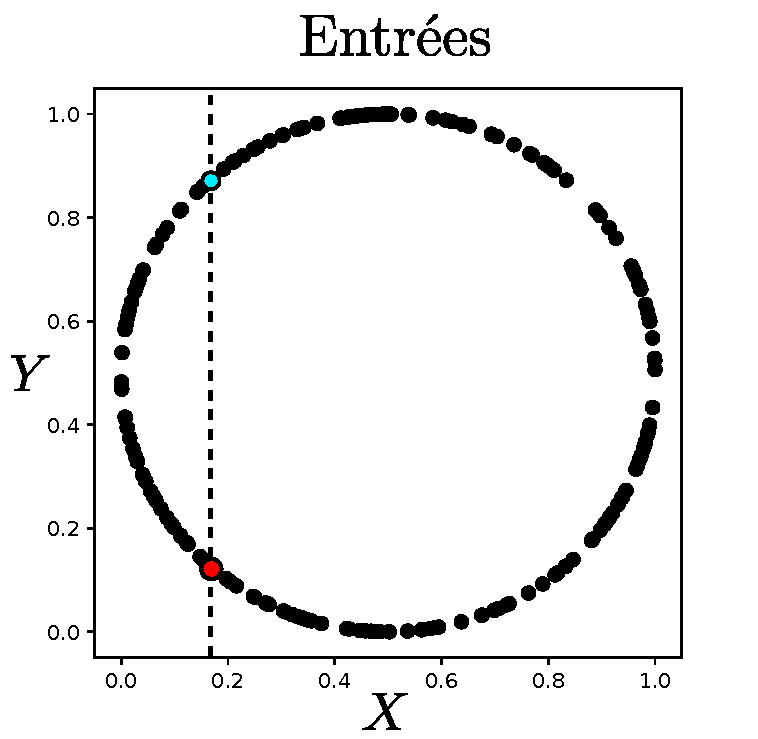
\includegraphics[width=0.8\textwidth]{2som_inp_noinformation}
\end{minipage}
\begin{minipage}{0.6\textwidth}
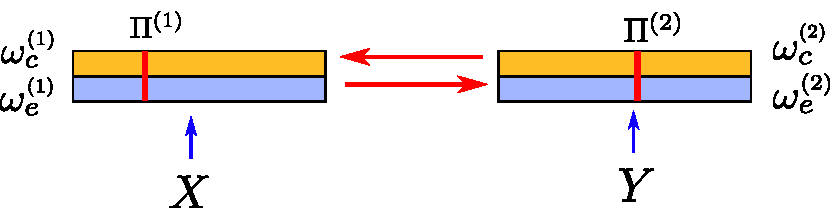
\includegraphics[width=\textwidth]{2som_archi}
\end{minipage}
\caption{A gauche, disposition des entrées dans l'exemple illustratif, sous forme de cercle. A droite, l'architecture de deux cartes en une dimension utilisée sur ces entrées dans ce chapitre pour illustrer les méthodes de représentation.\label{fig:exp}}
\end{figure}

\subsection{Représentations et indicateurs classiques des cartes de Kohonen}

Les cartes de Kohonen sont particulièrement associées à une facilité de représentation et de visualisation. Leur nombre réduit de prototypes et leur aspect topologique permet d'en tracer une représentation visuelle interprétable.
La manière la plus couramment utilisée de représenter une carte de Kohonen est de tracer les poids de ses prototypes, disposés dans le graphe (ligne ou grille) qu'est la carte. Deux exemples courants de représentation sont les suivants: 
\begin{itemize}
\item Le graphe qu'est la carte de Kohonen est représenté dans l'espace de ses positions (la grille d'indices $(i,j)$, ou une ligne indexée par $i$. Sur chaque noeud est tracé le poids correspondant. C'est le cas sur l'exemple de gauche en figure~\ref{fig:representation} dans lequel les poids des prototypes, qui sont des imagettes, sont affichés en chaque point de la grille. 
\item Lorsque les données traitées sont des points deux ou trois dimensions, les poids des prototypes peuvent être directement tracés dans l'espace $\mathbb{R}^2$ ou $\mathbb{R}^3$. Ces poids sont reliés en fonction des positions des n\oe{}uds dans la carte, montrant ainsi la déformation de la carte dans l'espace d'entrée, c'est le cas sur l'exemple de droite en figure~\ref{fig:representation} pour une grille en deux dimension.
\end{itemize}
Nous utiliserons des représentations adaptées au cas d'une architecture à plusieurs cartes à partir de ces deux modes de représentation.

\begin{figure}
\begin{minipage}{0.5\textwidth}
\centering
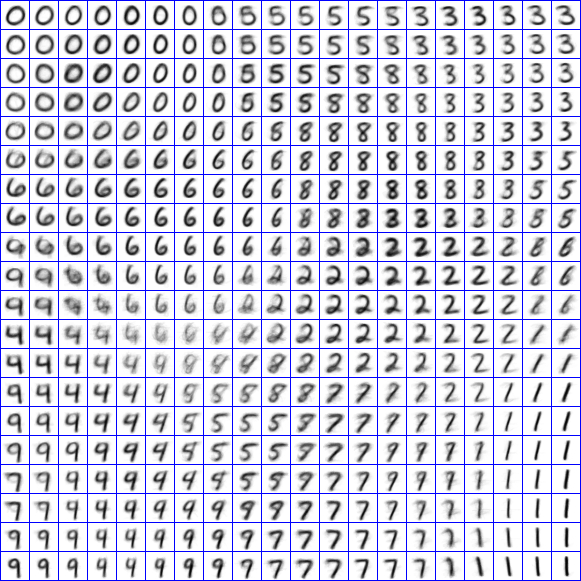
\includegraphics[width=0.5\textwidth]{digits.jpg}
\end{minipage}
\begin{minipage}{0.5\textwidth}
\centering
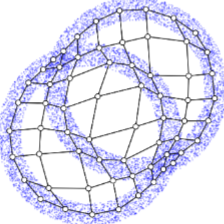
\includegraphics[width=0.5\textwidth]{points.png}
\end{minipage}
\caption{Représentations possible des poids d'une carte de Kohonen classiques, dans le cas d'entrées sous forme d'imagettes ou de points en deux dimensions.\label{fig:representation}}
\end{figure}

\subsection{Limites des représentations classiques dans le cas d'une architecture CxSOM}

Utilisons d'abord les représentations classiques mentionnées ci-dessus pour tracer les poids de chacun des cartes d'une architecture CxSOM à la fin de l'apprentissage.
La fin de l'apprentissage est définie comme le moment où les poids ont convergé vers une organisation restant stable au cours des itérations $t$.
La figure~\ref{fig:weights} présente le tracé des poids des deux cartes de l'exemple.
La courbe orange correspond aux poids externes des cartes, se dépliant sur chaque coordonnée $\inpx\m{1} = x$ et $\inpx\m{2} = y$ des points du cercle, appartenant chacune à $[0,1]$.
Ce tracé permet d'observer que les poids externes couvrent l'intervalle $[0,1]$, et sont organisés de façon monotone: ce comportement est celui qu'on attend dans une carte de Kohonen classique. Les poids contextuels, en bleu, ne présentent pas cette organisation monotone. Ils présentent toutefois une continuité: deux prototypes proches ont des poids proches. Le tracé des deux couches de poids nous informe donc sur le caractère continu de l'organisation de chacune de couches de poids. 

Notons que nous ne pouvons pas en tirer plus de conclusion: la représentation des poids de la figure~\ref{fig:weights} ne différencie pas les n\oe{}uds qui seront effectivement BMUs, des n\oe{}uds dits \emph{morts}.
Ces n\oe{}uds morts ont bien un poids, mais ne seront jamais BMUs.
Dans une carte de Kohonen classique, ces n\oe{}uds correspondent à des transitions, liant deux zones denses de l'espace d'entrée séparées par une zone sans points.
Par ailleurs, cette représentation concerne une seule carte. Nous ne pourrons pas tirer de conclusion sur l'influence des connexions entre cartes à partir de cette seule représentation.

Au regard des insuffisances des représentations classiques, que nous avons révélées sur un cas très simple de deux cartes mono-dimensionnelles, nous constatons qu'il est nécessaire de trouver un moyen de représenter l'architecture comme un tout. Nous devons ainsi définir des représentations qui montrent comment l'architecture de cartes est capable d'apprendre les relations entre les entrées multimodales.

\begin{figure}
\centering
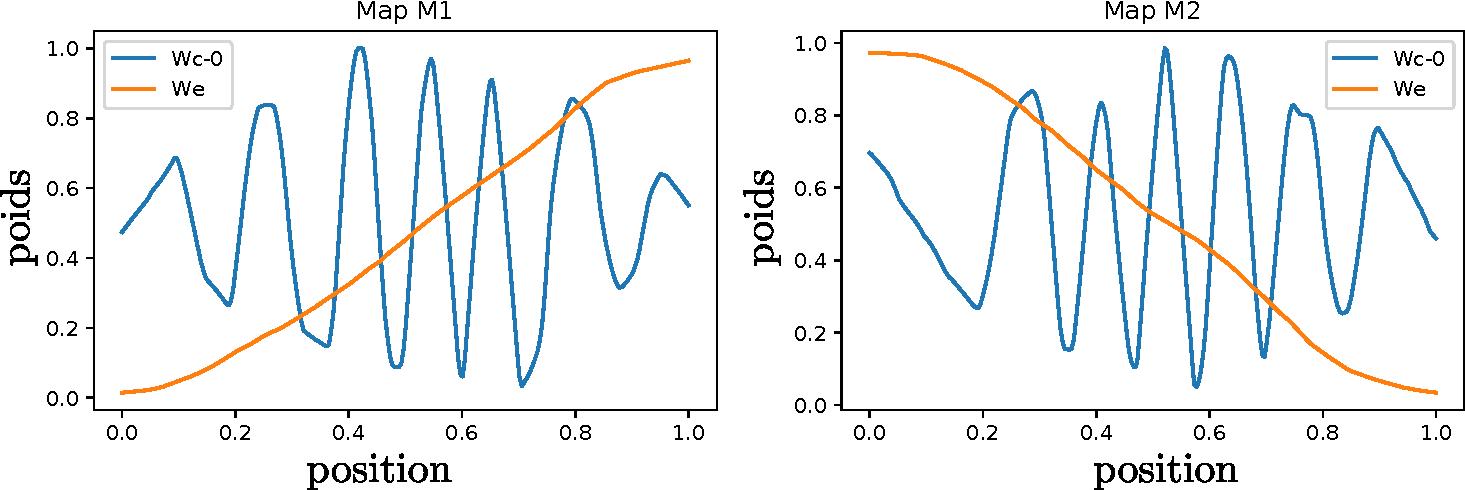
\includegraphics[width=0.9\textwidth]{weights_cercle1.pdf}

\caption{Représentation des valeurs des poids d'une carte au sein de CxSOM après apprentissage en fonction de leur position dans la carte. La seule représentation de ces poids ne suffit pas à savoir comment la carte se comporte.\label{fig:weights}}
\end{figure}

Suite aux limites montrées par les méthodes de représentation classiques utilisées dans le domaine des SOMs, ce chapitre propose plusieurs façons de représenter une carte au sein d'une architecture.
Nous présenterons en premier lieu le formalisme décrivant les cartes et leurs entrées multimodales associées ainsi que la méthode expérimentale que nous utiliserons pour toutes les expériences présentées dans cette thèse. \'A partir de ce formalisme, nous proposerons plusieurs représentations permettant de comprendre et représenter ce que calcule une architecture CxSOM sur les données d'entrées. Ces représentations seront illustrées sur un exemple minimal de deux cartes pour faciliter la compréhension. Nous utiliserons ces méthodes dans les chapitres suivants pour analyser le comportement des cartes.

\section{Formalisation statistique des entrées et sorties des cartes}

Nous introduisons dans cette section un formalisme traitant les éléments des cartes et les entrées en tant que variables aléatoires. 
Ce formalisme possède à la fois l'avantage de clarifier les représentations et de permettre le développement d'indicateurs statistiques sur l'apprentissage effectué par les cartes.

\subsection{Formalisation des entrées}

Plaçons-nous dans le cas général d'une architecture de $N$ cartes pour formaliser davantage.
Nous considérons des entrées multimodales tirées d'un ensemble d'espaces d'entrée $\mathcal{D}\m{1},\cdots,\mathcal{D}\m{n}$. Chaque espace $\mathcal{D}\m{i}$ est une modalité.
Les observations multimodales que l'on cherche à apprendre par l'architecture de cartes sont notées $(\inpx\m{i} \in \mathcal{D}\m{i}, i = 1 \cdots N)$.

Nous choisissons de modéliser ces entrées $\inpx\m{i}$ comme des \emph{variables aléatoires}.
Chaque variable aléatoire possède une distribution $p\m{i}$ sur $\mathcal{D}\m{i}$.
Nous notons $\mathbf{\inpx} = (\inpx\m{1}, \cdots, \inpx\m{n})$ la variable aléatoire jointe.
Cette variable appartient à l'espace $\mathcal{D}\m{1} \times \cdots \times \mathcal{D}\m{n}$.
A chaque pas de temps, un vecteur $\mathbf{\inpx} = (\inpx\m{1}_t, \cdots , \inpx\m{n}_t)$ est présenté à l'architecture: il s'agit d'une réalisation de la variable jointe $\mathbf{\inpx}$. 

En pratique, ces variables sont des observations, issues par exemple de capteurs d'un robot. Ces observations sont issues d'un environnement général et sont donc liées par des relations au sein de ce modèle d'environnement~: les variables $\inpx\m{i}$ ne sont pas des variables indépendantes.
Nous introduisons la notion de \emph{modèle d'entrées} se rapportant à cette dépendance entre variables.
Le modèle d'entrée fait référence au modèle d'environnement permettant de générer les entrées multimodales fournies en entrées. Dans l'exemple d'illustration, les modalités sont les abscisses $\inpx\m{1} = x$ et les ordonnées $\inpx\m{2} = y$; le modèle d'entrées correspond au cercle, modélisé par une équation.

Le but de l'apprentissage non-supervisé par des cartes de Kohonen classiques est d'apprendre une représentation discrète de l'espace d'entrée.
Avec CxSOM, nous chercherons à la fois à apprendre un représentation discrète des espaces d'entrée mais aussi à apprendre une représentation du modèle d'entrées.

Les tracés que nous développerons dans cette section ont pour but de mesurer comment ce modèle d'entrées est représenté par l'architecture. 

\subsection{Formalisation du modèle d'entrée par une variable cachée}

Nous cherchons à évaluer expérimentalement la capacité du modèle CxSOM à apprendre à partir d'un environnement multimodal. Dans ce cadre expérimental particulier, nous choisissons des modèles d'entrées dont les relations sont connues.
Ces modèles peuvent être paramétrisés par une variable multidimensionnelle $U$. Les modalités sont alors définies comme des fonctions de cette variable~:
$\inpx\m{i} = f\m{i}(U)$
$U$ est une nouvelle variable aléatoire, décrivant l'ensemble des paramètres du modèle.

Pour que la variable $U$ conserve toute l'information sur le modèle d'entrées, la fonction $(f\m{1}, \cdots, f\m{n})$ : $(\inpx\m{1}, \cdots \inpx\m{n})\rightarrow U$ doit être une bijection. Toute valeur d'entrées jointes correspond à un seul $U$, toute valeur de $U$ renvoie à une seule valeur d'entrées jointes. 
La définition de $U$ peut aussi être considérée comme un cas particulier de réduction de dimension du modèle, dans lequel la variable $U$, de dimension plus faible que $\mathbf{X}$, réduit la dimension des entrées sans perte d'information.


La variable $U$ s'interprète par l'existence d'une variété de dimension inférieure ou égale à la dimension des entrées, sur lesquelles les entrées multimodales se trouvent.

Des travaux récents font l'hypothèse que des variables en grande dimension telles que des images sont en pratique positionnées sur des variétés de dimension plus faible \cite{Pless2009ASO}.
Les algorithmes d'apprentissage de ces entrées font du \emph{manifold learning}, de l'apprentissage de variété, qui correspond à une réduction de dimension non-linéaire des entrées.
Des entrées multimodales en haute dimension seront positionnées sur un manifold de dimension inférieure ou égale. D'après cette observation, manifold de dimension probablement inférieur.
La modélisation des variables multimodales en passant par leur représentation par une variété inférieure est ainsi un cadre d'expériences général, en faible dimension dans nos travaux.
Les travaux de réduction de dimension non-linéaire permettent d'extraire des structure dans les données.
Ainsi, bien que nos travaux se concentrent sur des données en faible dimension, la représentation paramétrique est généralisable à des données de plus grande dimension.
%Isomap, Locally Linear Embedding, Laplacian Eigenmaps, Semidefinite Embedding, etc : algo de réduction de dim non linéaire. 
% t-SNE exemple mnist ? 
%PCA : réduction linéaire, on perdra de l'info.
\begin{figure}
    \centering
    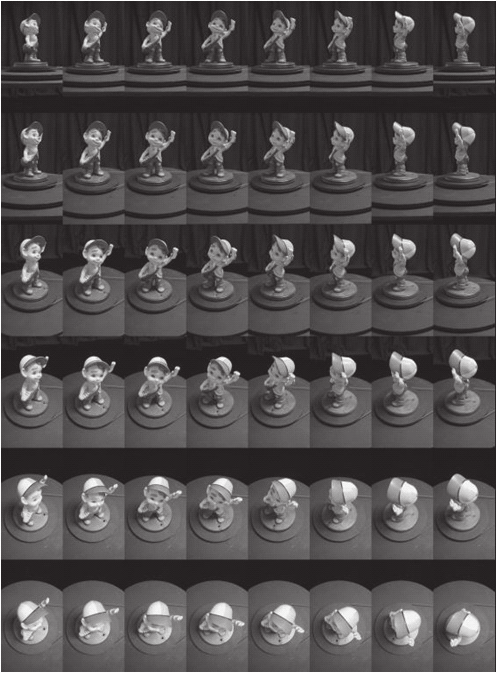
\includegraphics[width=0.4\textwidth]{pless-000.png}
    \caption{Ensemble d'images représentant une statuette sous différents angles de vue. Toutes les images, de grande dimension, sont situées sur un manifold 3D sous-jacent représentant la rotation de la caméra. Source~:~\cite{Pless2009ASO}}
\end{figure}


Dans le cas d'exemple, $\mathbf{X} = (\inpx\m{1},\inpx\m{2})$ est un vecteur aléatoire prenant comme valeurs les coordonnées cartésiennes des points du cercle de centre $x_c,y_c = 0.5,0.5$ et de rayon $r = 0.5$.
En définissant une variable $U$ scalaire à valeurs dans $[0,1]$, ces variables aléatoires peuvent maintenant s'écrire, selon l'équation paramétrique du cercle~:
\begin{equation}
 \begin{cases}
     \inpx\m{1}= x_c + r  \cos(2\pi U)\\
     \inpx\m{2} = y_c + r \sin(2 \pi U)
    \end{cases}\,.
\end{equation}

$U$ représente ici l'angle du point sur le cercle (à un facteur $2\Pi$ près). Les données 2D sont situées sur une variété de dimension 1.
Ce modèle n'étant pas fourni à l'architecture de cartes lors de l'apprentissage, il s'agit d'un modèle \emph{latent}.
Nous cherchons, par l'architecture de cartes, à apprendre les entrées et les relations entre entrées~: nous cherchons donc à extraire une structure dans le modèle latent. La relation entre $U$ et $\mathbf{X}$ est bijective~; de ce fait, étudier comment l'architecture de cartes a appris $U$ est équivalent à étudier comment l'architecture a appris le modèle d'entrées.
Cet exemple est scalaire mais la représentation sous forme de variable cachée est générale à n'importe quel dimension et nombre d'entrées. En effet, toute configuration d'entrée multimodale dépend d'un environnement global. La variable $U$ correspond alors aux paramètres de cet environnement.
Néanmoins, dans le cas de variables non artificielles, cette variable d'environnement est inconnue.
Nous utiliserons donc la variable cachée $U$ uniquement dans les expériences sur données artificielles. Elle nous permettra d'étudier et de représenter comment les cartes apprennent le modèle d'entrées.

\begin{figure}
\centering
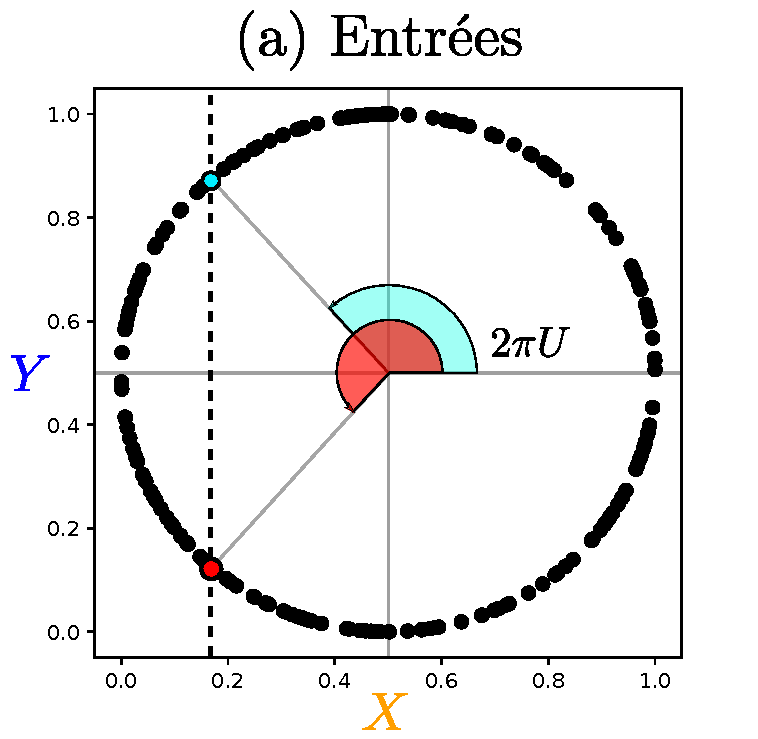
\includegraphics[width=0.4\textwidth]{2som_inp.pdf}
\caption{Représentation choisie pour le cercle. Le modèle auxquelles appartiennent les modalités $\inpx\m{1}$ et $\inpx\m{2}$ est représenté par la variable $U$. \label{fig:U}}
\end{figure}



\subsection{Démarche expérimentale}

Afin d'étudier le comportement de la carte à n'importe quel instant $t$ de l'apprentissage, nous effectuons une phase de \emph{test}, décrit en figure~\ref{fig:flowchart}.
Lors de cette phase de test, des entrées sont présentées à la carte, mais seul le processus de recherche de la best matching unit est réalisé, les poids des cartes ne sont pas mis à jour. Cet étape génère un ensemble de réponses de la carte aux entrées présentées.
Les entrées utilisées lors du test sont un échantillon de taille 1000 de la variable aléatoire $(\inpx\m{1}, \cdots, \inpx\m{n})$.
La distribution des entrées test est identique à la distribution des entrées d'apprentissage ayant servi au dépliement de la carte.

Nous formalisons non seulement les entrées mais aussi chaque élément de réponse des cartes d'une architecture comme une variable aléatoire.
Un élément de réponse d'une carte est une valeur régissant aux entrées lors d'une itération: positions du BMU, activité, poids du BMU.
Nous choisissons notamment de s'intéresser aux position des BMUs $\bmu\m{1}, \cdots, \bmu\m{n}$ et à leurs poids $\w\ext\m{1}(\bmu\m{1})$ et $\w\ext\m{2}(\bmu\m{2})$.
La valeur de ces éléments est indépendante entre deux itérations de test, car les poids ne sont pas mis à jour.
Grâce à cette indépendance entre itérations, les valeurs obtenues lors d'une phase de test forment un échantillon de la variable aléatoire jointe : 
$$(\underbrace{\inpx\m{1}, \cdots, \inpx\m{n}, U,}_{\text{Entrées}} \underbrace{\bmu\m{1}, \cdots, \bmu\m{n}, \w_e\m{1}(\bmu\m{1}), \cdots, \w_e\m{n}(\bmu\m{n})}_{\text{Eléments de réponse}})$$

Les composantes de cette variable jointe ne sont pas indépendantes. Maintenant que la démarche expérimentale est formalisées, les représentations présentées par la suite sont simplement des tracés de dépendances au sein d'un échantillon de test entre composantes de la variable jointe définie ci-dessus.

Les variables d'entrées sont à valeurs continues et $\bmu$ à valeurs discrètes, correspondant aux 500 n\oe{}uds d'une carte. Nous considérerons cependant $\bmu$ comme une variable continue plutôt qu'une grandeur discrète. En effet, l'ensemble des positions du BMU correspondent à une discrétisation de l'espace continu $[0,1]$, et sont ordonnées. Le déplacement par relaxation n'est pas limité aux positions discrètes des BMUs. Les variables aléatoires considérées sont bien à valeurs continues. Le formalisme par variable aléatoires permettra aussi d'utiliser des outils et métriques issus de la théorie de l'information pour qualifier l'organisation des cartes au sein de l'architecture, ce que nous ferons dans le chapitre~\ref{chap:indicateur}.

\begin{figure}
\centering
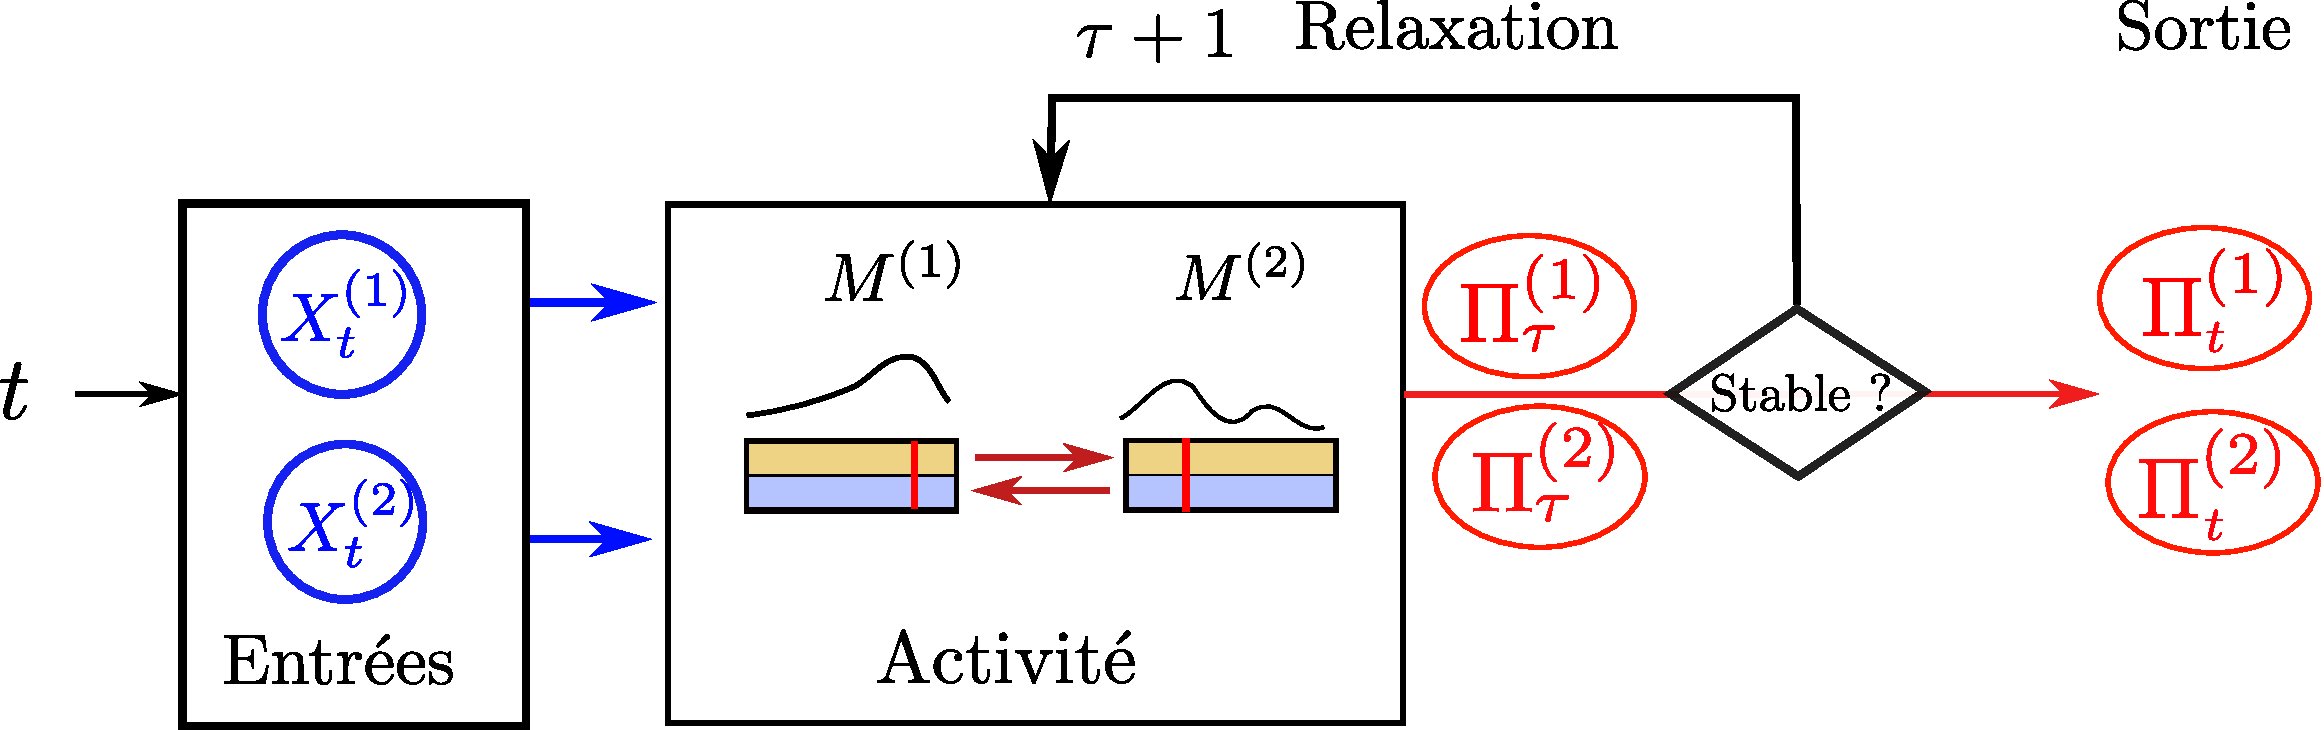
\includegraphics[width=0.85\textwidth]{tests_2maps.pdf}
\caption{Schéma décrivant une étape de test. Un test consiste à présenter successivement des réalisations de $\mathbf{X}$, notées $(\inpx\m{1}_t,\inpx\m{2}_t)$. Nous laissons le processus de relaxation stabiliser les BMUs. Quand la stabilité est atteinte, la valeur des positions de BMU $\bmu\m{1}_t$ et $\bmu\m{2}$ est obtenue. Un échantillon de test complet est ainsi obtenu en présentant un ensemble de réalisations de $\mathbf{X}$. Les poids ne sont pas mis à jour entre chaque itération, ce qui permet de considérer une phase de test comme un échantillonnage de la variable aléatoire $()\inpx\m{1},\inpx\m{2}, U, \bmu\m{1}, \bmu\m{2}$) }
\label{fig:flowchart}
\end{figure}

\section{Représentations graphiques}
\`A partir des échantillons de test, nous proposons dans cette section les représentations graphiques que nous utiliserons pour évaluer expérimentalement les architectures de cartes.
Ces représentations sont toute un tracé de dépendances entre des composantes de la variable $$(\inpx\m{1}, \cdots, \inpx\m{n}, U, \bmu\m{1}, \cdots, \bmu\m{n}, \w_e\m{1}(\bmu\m{1}), \cdots, \w_e\m{n}(\bmu\m{n}),U)$$ dont un échantillon est obtenu lors du test.
% Nous proposons d'abord une représentation pour évaluer la qualité de quantification vectorielle effectuée par une carte de l'architecture. Nous présenterons ensuite des représentations nous permettant de comprendre comment le modèle d'entrées est appris par l'architecture CxSOM.

\subsection{Erreur de quantification d'une modalité dans chaque carte}

La première fonction d'une carte de Kohonen est de réaliser une tâche de quantification vectorielle sur son entrée externe. Au sein d'une architecture de cartes, nous nous attendons à ce que chaque carte extraie une représentation de la modalité qu'elle prend en entrée externe.
Afin de mesurer cette qualité de quantification vectorielle au sein d'une carte dans CxSOM, nous traçons le nuage de points correspondant au poids externe du BMU $\w_e(\bmu\m{i})$ en fonction de l'entrée externe présentée $\inpx\m{i}$. Une carte effectue une quantification vectorielle correcte si ce nuage de points est proche de la fonction identité.
Ces tracés sont réalisés en figure~\ref{fig:erreur} pour l'expérience exemple. Ces tracés s'approchent de l'identité: la quantification des entrées est correctement réalisée.
On pourrait mesurer une erreur quadratique moyenne pour déterminer numériquement cette erreur de quantification mais la représentation en nuage de points est, à défaut d'être quantitative, plus qualitative. En effet, ici, on observe que le nuage montre une structure "filamenteuse". Nous reviendrons sur ce point par la suite, nous contentant de souligner ici que la représentation graphique exprime une propriété que la simple mesure d'erreur n'aurait pas mise en évidence. 

Cette représentation nous informe ainsi sur la qualité de quantification dans une seule carte relativement à une seule modalité. Cette seule représentation est insuffisante à elle seule pour comprendre plus en détail le comportement d'une architecture de cartes~: il nous faut également définir des méthodes de représentation permettant d'évaluer comment la structure globale du modèle d'entrées est apprise par l'architecture dans son ensemble.

\begin{figure}
    \centering
    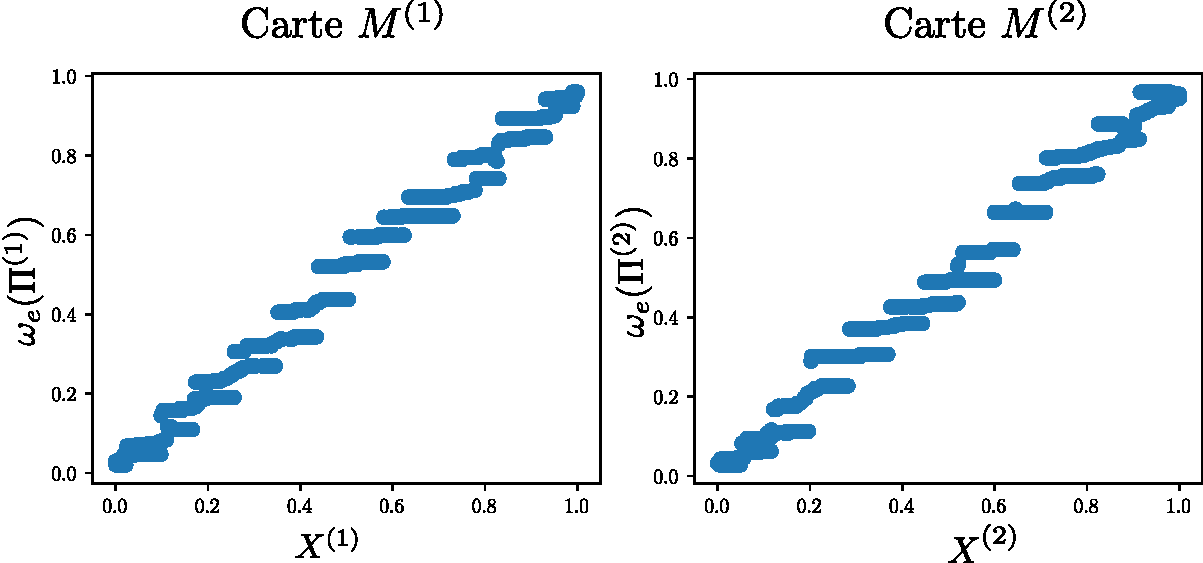
\includegraphics[width=0.7\textwidth]{w_x.pdf}
    \caption{Poids du BMU dans chaque carte en fonction de l'entrée présentée. On s'attend à des tracés proches de l'identité, montrant que le poids du BMU d'une carte est une bonne représentation de l'entrée. Sur ce graphique, on se rapproche effectivement de la fonction identité, cependant, une faible erreur est observée. On observe également un découpage des poids en bandes.\label{fig:erreur}}
\end{figure}


\subsection{Représentation cartographique des valeurs d'entrées préférentielles des BMUs}

En biologie, les aires du cortex cérébral sont cartographiées en faisant varier le motif d'entrée dans son espace, et en indiquant pour chaque neurone la valeur d'entrée préférentielle à laquelle il réagit. Cela donne alors une représentation cartographique où des valeurs de l'espace d'entrée sont tracées par rapport à la position sur le substrat neuronal du neurone qui y réagit.
Par exemple, une carte corticale est tracée pour l'aire visuelle primaire du cortex cérébrale, l'aire v1, en figure~\ref{fig:v1_repr}.

Un échantillon test donne un ensemble de valeurs de variable jointe $(\inpx\m{1}, \cdots, \inpx\m{n}, \bmu\m{1},\cdots, \bmu\m{n})$.
Dans la même idée que les cartes corticales, nous tracerons à partir de l'échantillon de test le nuage de points correspondant à la valeur de l'entrée $\inpx\m{i}$ d'une carte par rapport à la position du BMU $\bmu\m{i}$.
Cette représentation permet d'analyser la quantification des entrées par la carte. 
On s'attend à ce que les points soient proches de la courbe des poids externes de la carte $M\m{i}$.
Ce tracé fait également apparaître les zones dans lesquelles les neurones ne sont jamais best matching unit, les \emph{zones mortes}.
En plus des couples $(\bmu\m{i},\inpx\m{i})$, nous traçons également les entrées externes des autres cartes en fonction de $\bmu\m{i}$ : $(\bmu\m{i},\inpx\m{j})$.
Enfin, sur le même graphique, nous mettons ces valeurs d'entrées externes en relation avec les poids de la carte $M\m{i}$ en traçant les poids externes et contextuels de la carte $M\m{i}$ en fonction de leur position.
Une représentation cartographique fait ainsi apparaître les poids externes et contextuels d'une carte de l'architecture. A ces poids s'ajoutent plusieurs nuages de points correspondant aux valeurs d'une entrée $\inpx\m{j}$ en fonction du BMU de la carte $M\m{i}$, $\bmu\m{i}$.

En figure~\ref{fig:inputs}, nous avons ainsi tracé cette représentation cartographique pour l'exemple à deux cartes.
Nous y voyons deux nuages de points: $(\bmu\m{1},\inpx\m{1})$ et $(\bmu\m{1},\inpx\m{2})$ issus de l'expérience sur les deux cartes, ainsi que deux courbes: les poids externes et contexuels de la carte $M\m{1}$.
Deux valeurs issues de l'échantillon de test sont mise en évidence en couleur rouge et bleue sur chaque graphique. Un point de même couleur correspond à la même itération de test dans chaque graphique. Ces deux points partagent la même abscisse, donc l'entrée $\inpx\m{1}$ est la même pour ces deux échantillons. Par contre, leur ordonnée est différente: $M\m{2}$ reçoit donc une entrée $\inpx\m{2}$ différente entre de ces deux itérations.

Ce tracé nous permet d'abord d'observer que les points $(\bmu\m{1},\inpx\m{1})$ sont proches de la courbe de poids externe: le poids d'un BMU est proche de l'entrée qui a été présentée, le poids du BMU est donc une bonne approximation de cette entrée. Cela permet de conclure que la quantification vectorielle est bien réalisée dans cette carte sur les entrées externes, comme le montrait déjà la figure~\ref{fig:erreur}.

Tracer les échantillons de test permet ensuite d'observer la répartition des BMUs sur la carte. Les courbes de poids externes de la carte dans CxSOM (c) et de la carte indépendantes (b) sont indifférenciables; par contre, l'affichage de l'échantillon de test fait apparaître des zones mortes, sans BMUs. Nous observons ainsi que la carte au sein de CxSOM est découpée en plusieurs zones dans lesquelle les unités sont BMUs, séparées par des petites zones mortes. Ce tracé permet donc d'identifier un comportement nouveau dans une architecture de cartes, par rapport à une carte classique.

Les nuages de points $(\bmu\m{1},\inpx\m{1})$ et $(\bmu\m{1},\inpx\m{2})$ nous permettent d'observer quelles valeurs d'entrées sont codées dans les zones observées sur les positions des BMUs.
Nous observons notamment qu'une zone encode pour un intervalle de valeurs spécifique pour le couple $(\inpx\m{1},\inpx\m{2})$ et non seulement pour l'entrée externe de la carte, comme ce serait le cas dans une carte seule (b). Les points rouges et bleus illustrent ce comportement.
Ces échantillons correspondent à la même valeur d'entrée externe présentée à $M\m{1}$, mais $\inpx\m{2}$ est différent.
Dans la carte indépendante, le BMU sera identique pour ces deux valeurs.
Sur la figure (c), le point rouge et le point bleu ont leurs BMUs dans deux zones adjacentes, mais séparées, sur la carte.

La représentation des valeurs d'entrées $\inpx\m{j}$ selon la position du BMU $\bmu\m{i}$ permet ainsi d'identifier une répartition des BMUs sur une carte que nous ne pourrions pas observer en traçant simplement les poids.
Nous voyons notamment que la carte s'auto-organise en zones de BMUs, séparées par des zones mortes.
Les n\oe{}ds d'une zone réagissent à des valeurs spécifiques du couple d'entrées et non de seulement l'entrée externe.
Cette organisation en zone observée sur ce graphique traduit l'existence de deux échelles d'indices: une organisation primaire selon la valeur de l'entrée externe, et une organisation secondaire au sein des zones selon la valeur de l'entrée de l'autre carte.
Nous étudierons dans les chapitres suivants, grâce à cette représentation, si ce comportement se généralise pour différentes architectures et distributions d'entrées.

% Sur la figure (c), les BMUs appartenant à une même zone encodent les entrées $\inpx\m{1}$ ainsi que $\inpx\m{2}$ sur un intervalle particulier. Ce comportement diffère de celui de la carte simple (b). Dans cette carte, il n'y a pas de création de zones et un intervalle de position des BMUs encode deux intervalles distincts de valeurs concernant les entrées $\inpx\m{2}$.
% Les intervalles encodés par deux zones de BMUs adjacentes se recoupent: ce phénomène est illustré par le fait que les points rouges et bleus, ayant la même valeur de $\inpx\m{1}$, sont envoyés dans deux zones différentes.

% Ces valeurs peuvent être mises en relation avec celles de l'entrée $\inpx\m{2}$, également disposées selon $\bmu\m{1}$. Nous pouvons alors observer que deux zones adjacentes de la carte encodent des entrées proches selon $\inpx\m{1}$, mais très différentes pour $\inpx\m{2}$. Cela explique la séparation du point rouge et du point bleu dans deux zones.

\begin{figure}
    \centering
    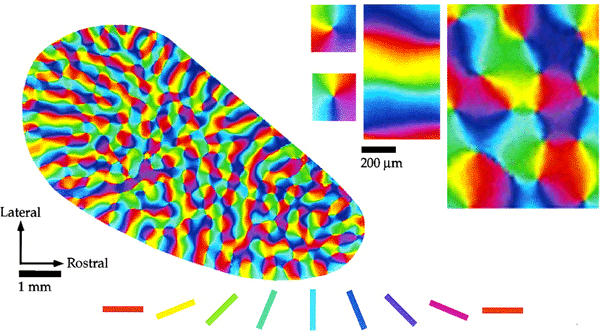
\includegraphics[width=0.7\textwidth]{v1.jpg}
    \caption{Carte corticale de l'aire cérébrale visuelle V1. Pour tracer cette représentation, un ensemble de traits de différentes orientation sont présentés en stimuli visuels au sujet, indiqués en bas de l'image. Le neurone réagissant à une entrée d'orientation particulière est coloré sur la carte de la couleur correspondante à l'entrée. Cette méthode permet de tracer des \emph{cartes corticales} d'une aire cérébrale \cite{Bosking1997OrientationSA}. \label{fig:v1_repr}}
\end{figure}

\begin{figure}
\begin{minipage}{0.27\textwidth}
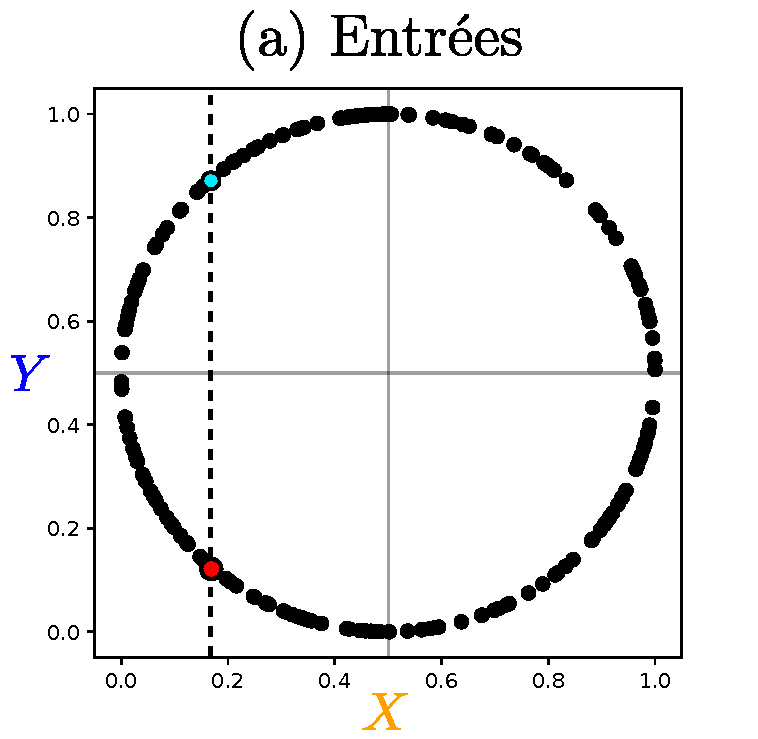
\includegraphics[width=\textwidth]{2som_inp_noU.pdf}
\end{minipage}
\begin{minipage}{0.34\textwidth}
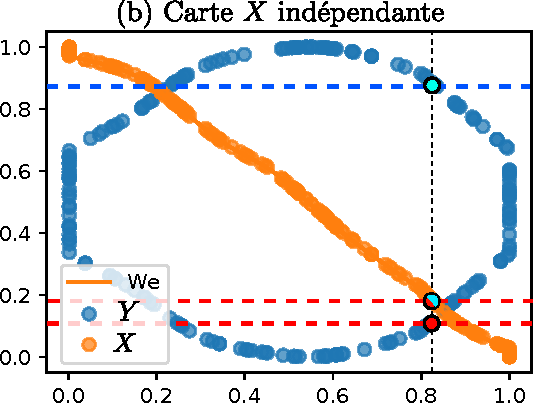
\includegraphics[width=\textwidth]{weights_2som_unco.pdf}
\end{minipage}
\begin{minipage}{0.38\textwidth}
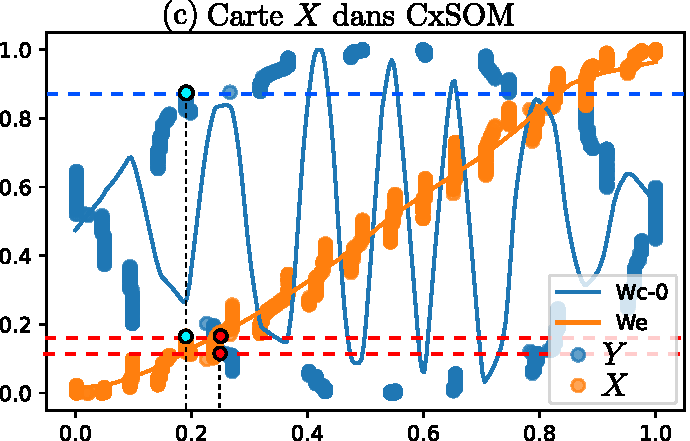
\includegraphics[width=\textwidth]{weights_2som.pdf}
\end{minipage}

\caption{Représentation des entrées $\inpx\m{1},\inpx\m{2}$ d'une architecture de deux cartes relativement au BMU de la carte $M\m{1}$ après apprentissage. Ces tracés mettent en valeur l'organisation des cartes, différentes dans le cas ou les cartes apprennent indépendemment leurs entrées~(b) ou sont connectées~(c). Les entrées correspondantes sont en figure~(a). Les points bleu et rouge reportés sur les tracés correspondent au même échantillon de test.\label{fig:inputs}}
\end{figure}

\subsection{Représentation de la variable cachée selon les positions des BMUs}

Nous avons vu lors de la représentation cartographique des entrées que chacune des cartes choisit son BMU  en fonction non seulement de son entrée externe, mais aussi de l'entrée de l'autre carte. Chaque carte s'organise donc en fonction du \emph{modèle d'entrée}, donc en fonction de $U$.
Afin de mettre en valeur ce comportement, nous tracerons les nuages de points représentant $U$ en fonction de la position $\bmu\m{i}$ du BMU d'une carte pour afficher comment la position du BMU traduit la relation entre les entrées.

En figure~\ref{fig:piu}, nous traçons $U$ en fonction de $\bmu\m{1}$ et $U$ en fonction de $\bmu\m{2}$.
Ce tracé montre $U$ comme une fonction de la position du BMU dans chaque carte, contrairement au cas ou les cartes ne sont pas connectées pour lequel deux valeurs de $U$ correspondent à un même BMU. Cela traduit bien le fait que chaque carte a appris une représentation du modèle d'entrée et non seulement de son entrée externe.
L'organisation de la carte dans CxSOM montre donc chaque position $\bmu$ codant pour une seule valeur de $U$, c'est à dire une seule position d'échantillon sur le cercle.
La représentation de $U$ selon la position du BMU d'une carte $\bmu\m{i}$ permet de représenter comment la carte $i$ a appris l'ensemble d'entrées $(\inpx\m{1},\inpx\m{2})$ et non seulement son entrée externe. Déterminer si l'architecture a appris le modèle d'entrées revient alors à vérifier si $U$ est une fonction de $\bmu$ dans chacune des cartes de l'architecture.

Cette représentation fait appararaître $U$ comme une fonction de $\bmu$ dans chaque carte. Ce comportement traduit le fait que les cartes s'organisent en fonction de tout le modèle d'entrée, non seulement de leur entrée externe. Il s'agit là d'un comportement que nous pouvons qualifier de comportement de base pour CxSOM. 

\begin{figure}
\centering
\includegraphics[width = 0.7\textwidth]{xu_yu_both.pdf}
\caption{Valeur de $U$ en fonction des valeurs du BMU $\bmu\m{i}$ dans chacune des cartes dans l'exemple d'illustration. Sur la première ligne, nous traçons la réponse de chaque carte à son entrée dans le cas ou les deux cartes ne sont pas connectées. Sur la deuxième ligne, nous traçons la réponse de chaque carte lorsqu'elles ont appris de façon jointe au sein de CxSOM.
$U$ apparaît alors comme une fonction de la position du BMU $\bmu\m{i}$ dans chaque carte, contrairement au cas ou les cartes apprendraient indépendamment sur les mêmes entrées. Cette relation fonctionnelle est symbolisée par les pointillés sur les tracés du bas. Les mêmes échantillons rouge et bleu mis en évidence en figure~\ref{fig:inputs} sont reportés sur les tracés.}
\label{fig:piu}
\end{figure}


\subsection{Dépliement d'une carte dans l'espace d'entrée multimodal}

Une représentation classique utilisée pour représenter une carte de Kohonen est de tracer les poids du graphe qu'est la carte dans l'espace de ses entrées, telle qu'en figure de droite en~\ref{fig:representation}. Dans CxSOM, chaque carte prend en entrée une seule des modalités. Par contre, grâce à l'échantillon de test, il est possible de représenter comment la carte se déplie dans l'espace de toutes les modalités.

Nous définissons alors une façon de représenter le dépliement d'une seule carte de CxSOM dans l'espace global des entrées. Dans l'exemple, il s'agit de représenter le dépliement de $M\m{1}$ dans l'espace des entrées $\inpx\m{1},\inpx\m{2}$.
Au lieu de s'appuyer sur les poids des cartes comme en~\ref{fig:representation}, nous utilisons les valeurs de l'échantillon de test. Nous traçons le nuage de poids correspondant au poids des BMUs: $\w_e\m{1}(\bmu\m{1},\w_e\m{2}(\bmu\m{2})$, puis relions ces points selon l'ordre de leurs positions dans la carte $M\m{1}$ ou $M\m{2}$. Ainsi, nous obtenons une représentation des cartes $M\m{1}$ ou $M\m{2}$ dépliées dans l'espace global des entrées. 
Notons que les unités mortes ne peuvent pas être représentées sur la carte. Nous ne représentons que les morceaux de cartes étant effectivement BMUs. 
Cette représentation est tracée en ~\ref{fig:distortion} pour l'exemple à deux cartes.


La carte représentant les poids externes des BMUs, on s'attend à ce que la forme du nuage de points corresponde à la structure des entrées.
Les tracés mettent en lumière les propriétés observées lors de la représentation cartographique des entrées, à savoir l'apparition de zones dans chaque carte. Les poids suivent la structure circulaire des entrées en découpant l'espace en zones. Les parties du cercle effectivement représentées par les poids sont réduites: le cercle est comme discrétisé en petits morceaux.
Dans l'exemple, on remarque la façon dont est parcouru l'espace dans chaque carte: en fonction de $x$ dans la carte $M\m{1}$, et en fonction de $y$ dans la carte $M\m{2}$. 
Cette représentation offre la possibilité  de visualiser comment une carte se déplie dans l'espace d'autres modalités.

\begin{figure}
    \begin{minipage}{0.49\textwidth}
    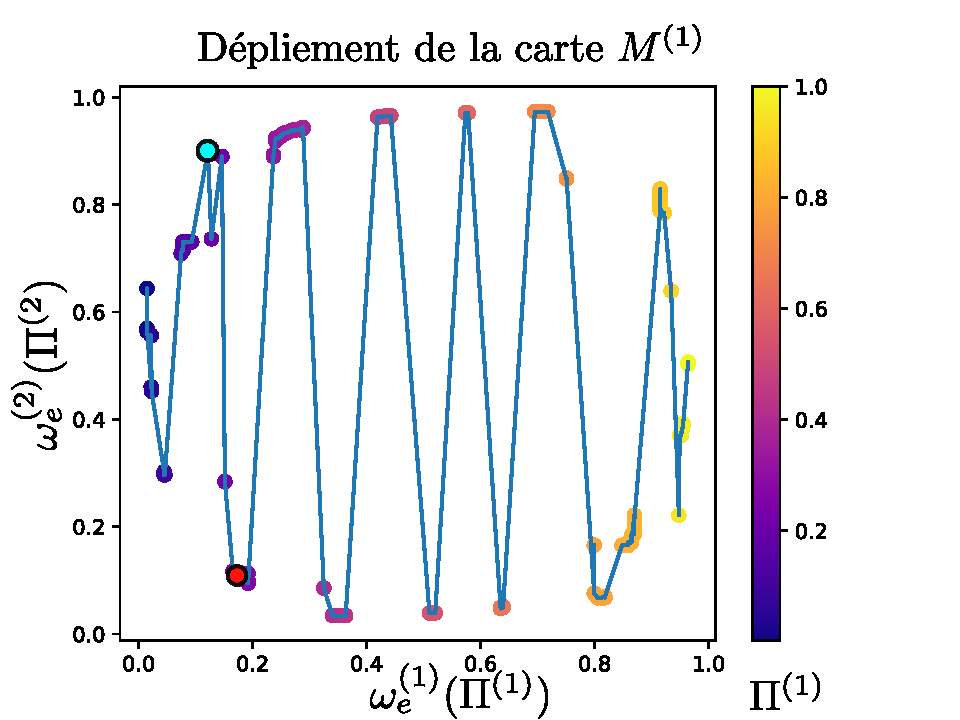
\includegraphics[width=\textwidth]{disto_cercle_M1.pdf}
    \end{minipage}
    \begin{minipage}{0.49\textwidth}
    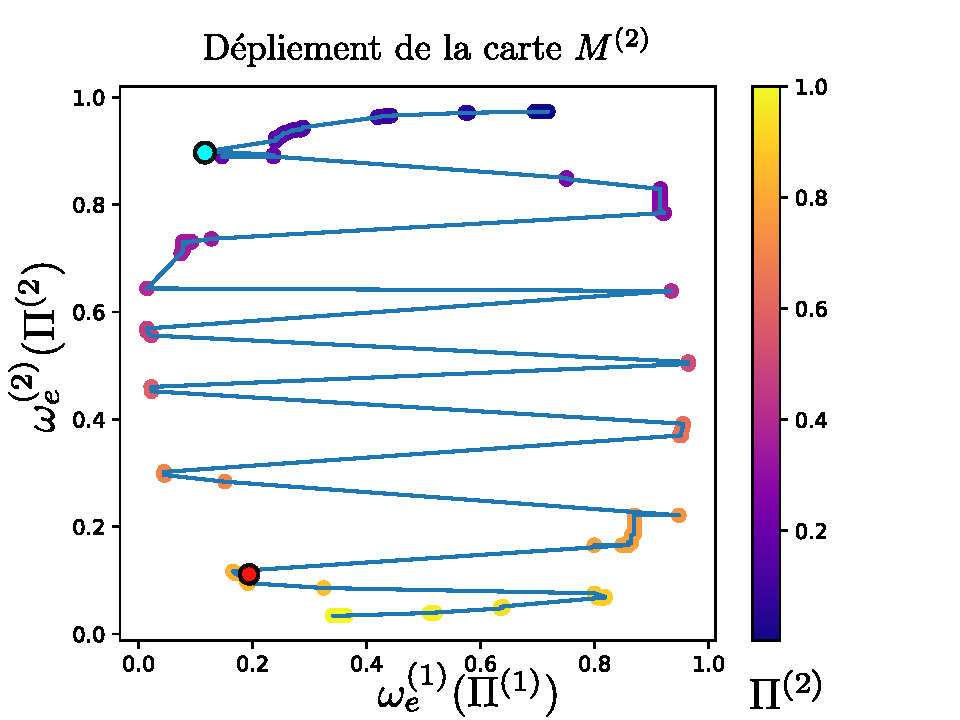
\includegraphics[width=\textwidth]{disto_cercle_M2.pdf}
    \end{minipage}
    \caption{Dépliement des cartes $M\m{1}$ et $M\m{2}$, reliés dans l'ordre de leurs positions selon $M\m{1}$ figure de gauche et $M\m{2}$ figure de droite. Le dépliement de chacune des cartes est alors représenté dans l'espace complet des entrées \label{fig:distortion}. L'indice du BMU est signalé par la carte de couleurs, différenciant ainsi les extrémités en 0 et 1 des cartes.}
    \end{figure}



\section{Utilisation du ratio de corrélation comme indicateur de l'apprentissage de $U$}

Nous cherchons à mesurer la dépendance fonctionnelle existant entre la variable $\bmu\m{i}$, les positions du BMU d'une carte, et la variable $U$ décrivant le modèle.
Le ratio de corrélation $\eta(\bmu\m{i},U)$ permet de mesurer un coefficient de dépendance non-linéaire entre deux variables, ce qui correspond à une relation fonctionnelle. Il atteint la valeur de 1 lorsque $U$ est fonction de la première variable $\bmu\m{i}$ et est nul lorsque les deux variables sont statistiquement indépendantes.
A ne pas confondre avec le coefficient de Pearsons $r$ qui mesure une dépendance linéaire. Cependant, eta rejoint r lorsque (??)

\subsection{Définition}

La mesure de la dépendance fonctionnelle entre deux variables $X$ et $Y$ peut se décomposer en deux étapes:
\begin{enumerate}
    \item Trouver une fonction $\varphi(X)$ qui approxime les valeurs de $Y$
    \item Mesurer la qualité de l'approximation.
\end{enumerate}

La fonction $\varphi$ considérée pour le calcul du ratio de corrélation est ici~:
\begin{equation}
    \varphi = \mathbb{E}(Y|X)
\end{equation}

Il s'agit bien d'une fonction de $X$. Un exemple de calcul de $\varphi$ est illustré en figure~\ref{fig:cr_box}, estimé par discrétisation des valeurs de $X$. Il s'agit en fait de la fonction approximant au mieux les valeurs de $Y$.

Le ratio de corrélation $\eta$ mesure ensuite la qualité de l'approximation des valeurs de $Y$ par la fonction $\varphi$ en faisant le rapport des variances de ces deux variables~:
\begin{equation}
    \eta(Y|X) = \frac{Var(\mathbb{E}(Y|X))}{Var(Y)}
\end{equation}

On peut mieux comprendre la signification de ce coefficient en modifiant un peu l'équation.
Par la définition des variances conditionnelles, on a 
$$Var(Y) = \mathbb{E}(Var(Y|X)) + Var(\mathbb{E}(Y|X))$$
Soit~:
$$\eta(Y|X) = 1 - \frac{\mathbb{E}(Var(Y|X))}{Var(Y)}$$
$\mathbb{E}(Var(Y|X))$ représente la moyenne des écarts de $Y|X=x_i$ à sa valeur moyenne en $x_i$ $\mathbb{E}(Y|X=x_i)$ pour une valeur de $X = x_i$ donnée. Lorsque la dépendance entre $Y$ et $X$ est fonctionnelle, les valeurs de $Y|X$ sont très proches de $\mathbb{E}(Y|X)$ pour chaque valeur de $X$ et $\mathbb{E}(Var(Y|X))$ est faible partout. La variance est nulle lorsqu'une valeur de $X$ correspond à un seul point pour $Y$, c'est à dire une relation fonctionnelle. Inversement, quand $Y$ et $X$ sont indépendantes, $\mathbb{E}(Var(Y|X)) = Var(Y)$ et le ratio de corrélation tombe ainsi à 0.
Le ratio de corrélation n'est pas symétrique. Par le fait qu'il s'appuie sur un rapport, il n'est pas sensible à une transformation linéaire de $Y$.

\begin{figure}
    \centering
    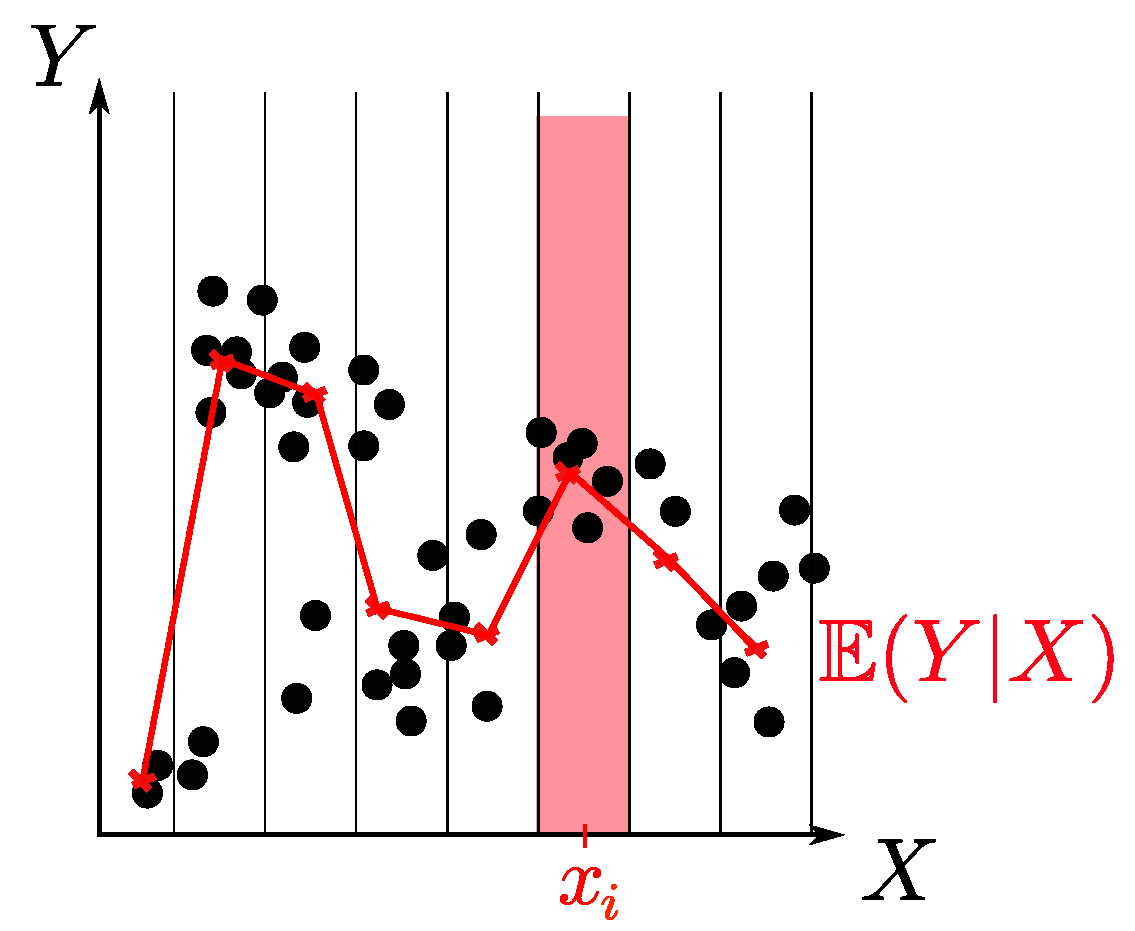
\includegraphics[width=0.6\textwidth]{boxes_CR.pdf}
    \caption{Exemple d'approximation non-linéaire de la relation entre $X$ et $Y$ par $\mathbb{E}(Y|X)$. Cette approximation est ici réalisée en discrétisant les valeurs de $X$. La valeur de la fonction pour chaque $x_i$ est alors la moyenne des valeurs de $Y$ sur l'intervalle considéré.}
\end{figure}

\subsection{\'Evolution du ratio de corrélation au cours de l'apprentissage des cartes CxSOM}

Nous utilisons le ratio de corrélation pour mesurer la dépendance fonctionnelle existant dans chaque carte entre les valeurs de $U$ et l'ensemble des BMU d'une carte $\bmu\m{i}$.
Les valeurs $\bmu\m{1}$ et $\bmu\m{2}$ étant des valeurs discrètes, $\mathbb{E}(U|\bmu\m{i})$ est estimée par la moyenne des valeurs de $U$ ayant pour BMU la même valeur $\bmu\m{i}$. 
En figure~\ref{fig:cr_xp}, nous traçons les distributions de $U$ en fonction de $\bmu\m{1}$ et $\bmu\m{2}$, dans le cas de l'architecture CxSOM et des cartes simples. Nous y représentons la fonction $\mathbb{E}(U|\bmu\m{i})$ en rouge.
Le ratio de corrélation apparaît ici comme une bonne mesure de la relation fonctionnelle existant entre $U$ et $\bmu$. Le ratio de corrélation est très proche de 1 dans chaque carte de CxSOM, traduisant le fait que $U$ est une fonction du BMU dans chaque carte.

La figure~\ref{fig:cr_bruit} présente les mêmes paramètres tracés dans le cas ou l'expérience est réalisée sur des données bruitées, en l'occurence un anneau. $U$ n'est alors plus vraiment une fonction du BMU, mais en reste proche. 
Le ratio de corrélation traduit correctement cette proximité et reste plus élevé dans chaque carte que pour une carte seule.

Enfin, nous tracons en figure~\ref{fig:cr_evol} l'évolution du ratio de corrélation sur les 200 premiers pas d'apprentissage de deux cartes sur un cercle, connectées et non connectées. Les mesures sont réalisées sur 10 expériences réalisées sur des distributions d'entrées identiques et moyennées.
Nous remarquons que $\eta$ reste inférieur dans le cas ou les cartes sont connectées que non connectées. 
Remarques:
\begin{itemize}
    \item Semble rester a peu près constant pendant tout l'apprentissage. Traduit le fait que dès le début de l'apprentissage, la relaxation différencie les BMUs en fonction des deux valeurs d'entrées, même quand les poids ne sont pas organisés.
    \item Pas d'information sur l'organisation topologique des poids ici: le coefficient ne traduit pas l'organisation de la carte.
    \item Grande variabilité de la valeur de $\eta$ entre les expériences, traduite ici par l'écart à la moyenne.
    \item On voit qu'entre la carte $M\m{1}$ et $M\m{2}$, $\eta$ prend une valeur bien différente, alors que la qualité de la relation est semblable. On peut donc difficilement utiliser $\eta$ de façon absolue, mais plutôt pour comparer des valeurs.
\end{itemize}

\begin{figure}
    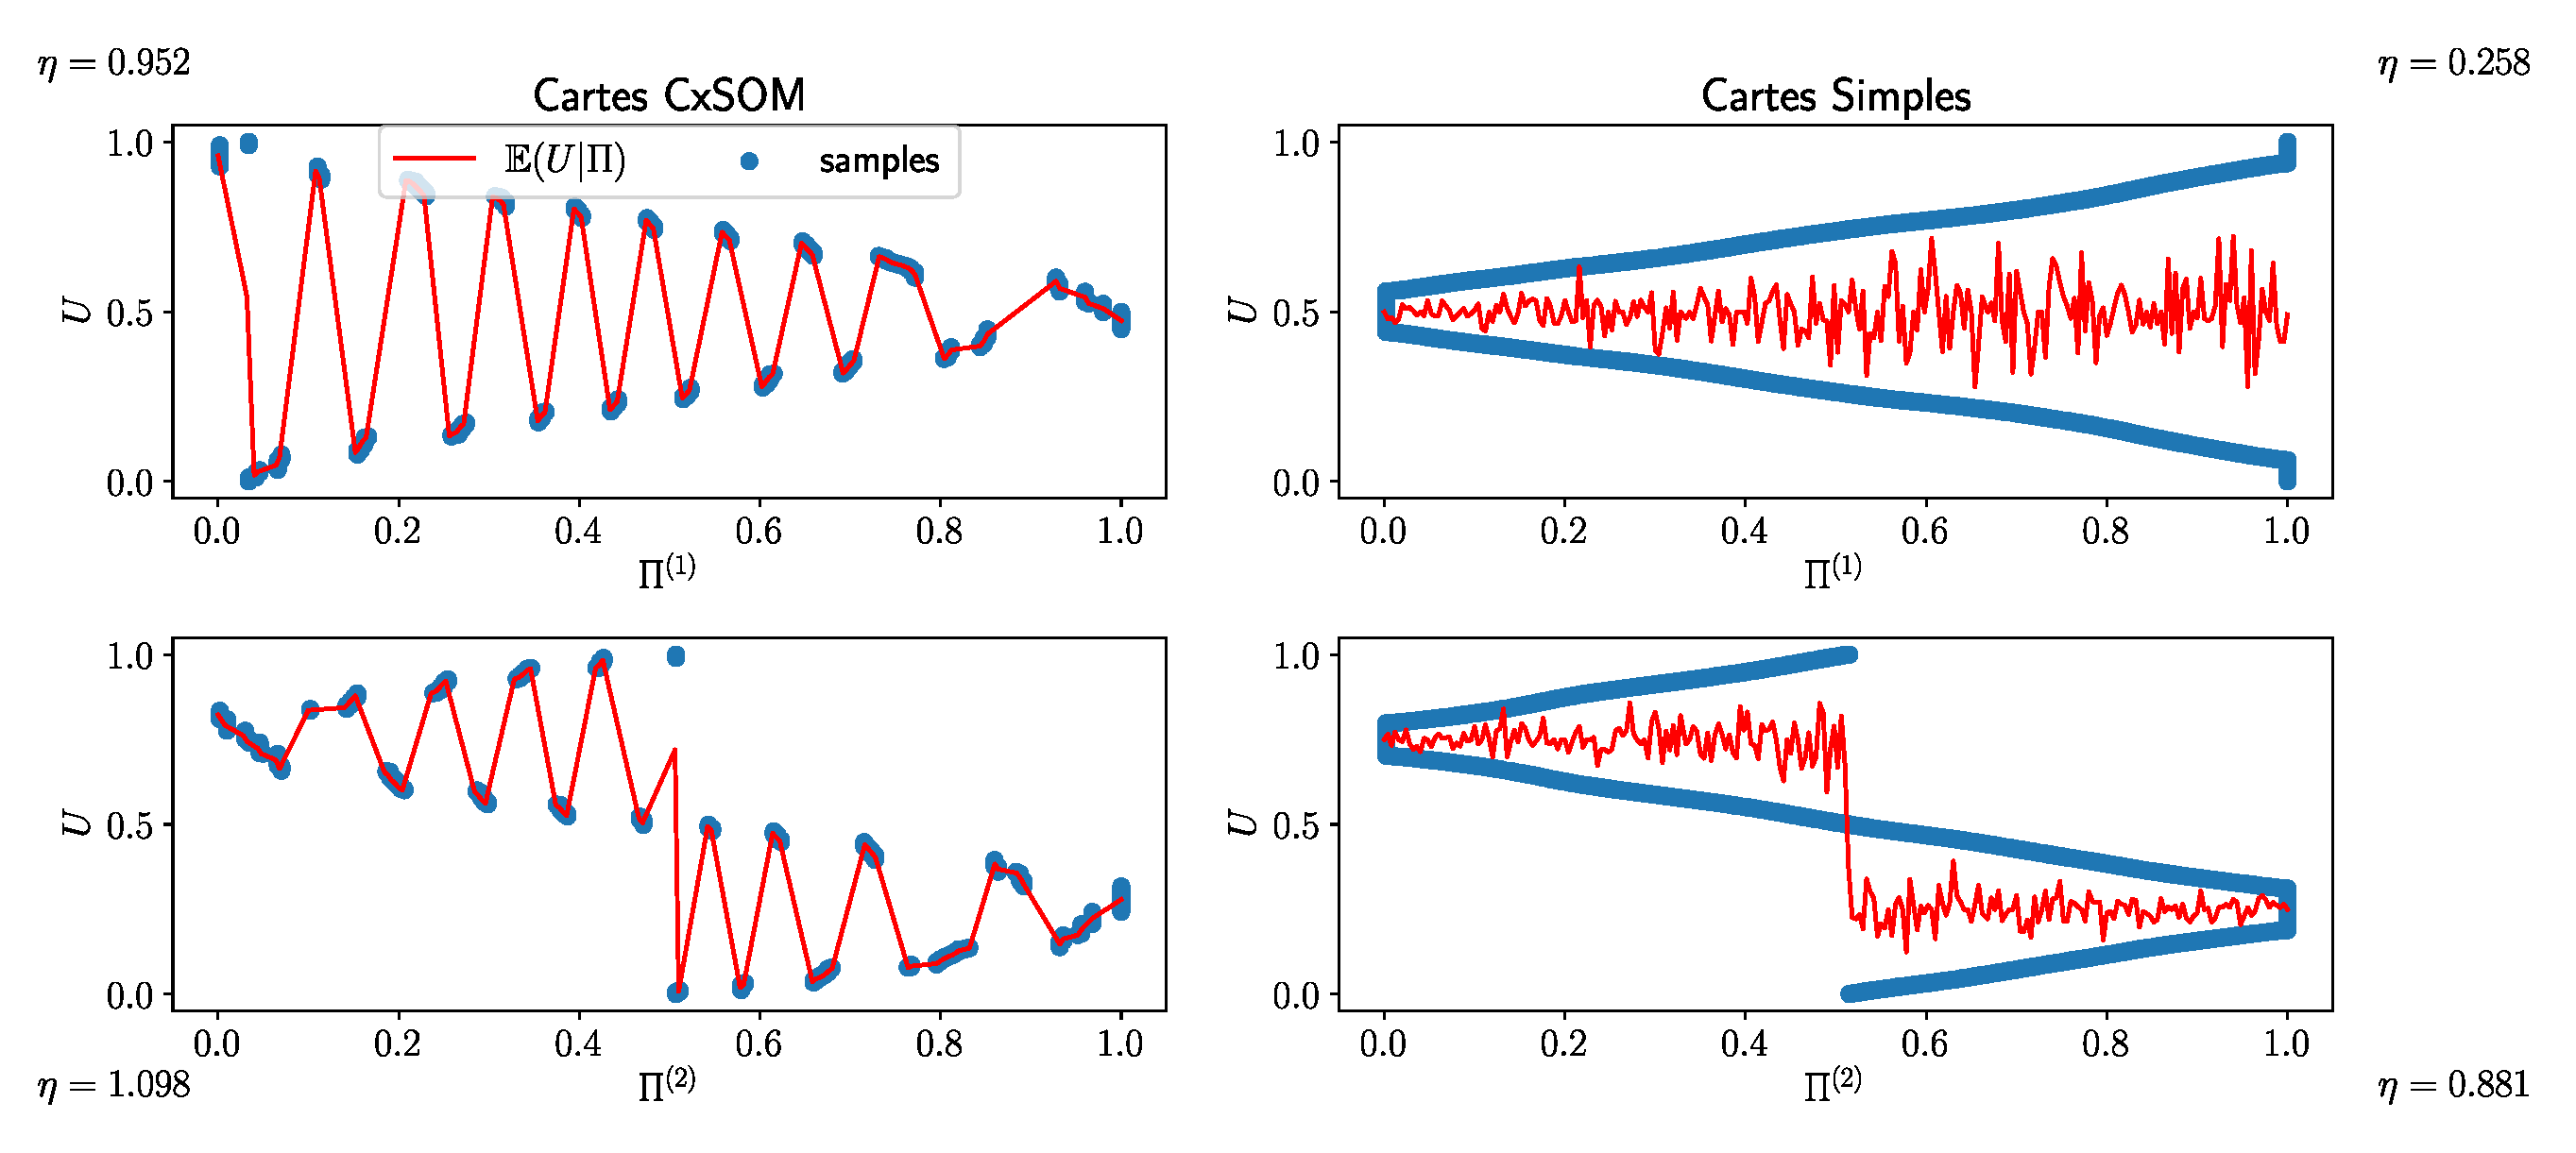
\includegraphics[width=\textwidth]{correlation_ratio_xp0.pdf}
    \caption{Tracé du ratio de corrélation sur cartes cxsom et cartes simples \label{fig:cr_xp}}
\end{figure}

\begin{figure}
    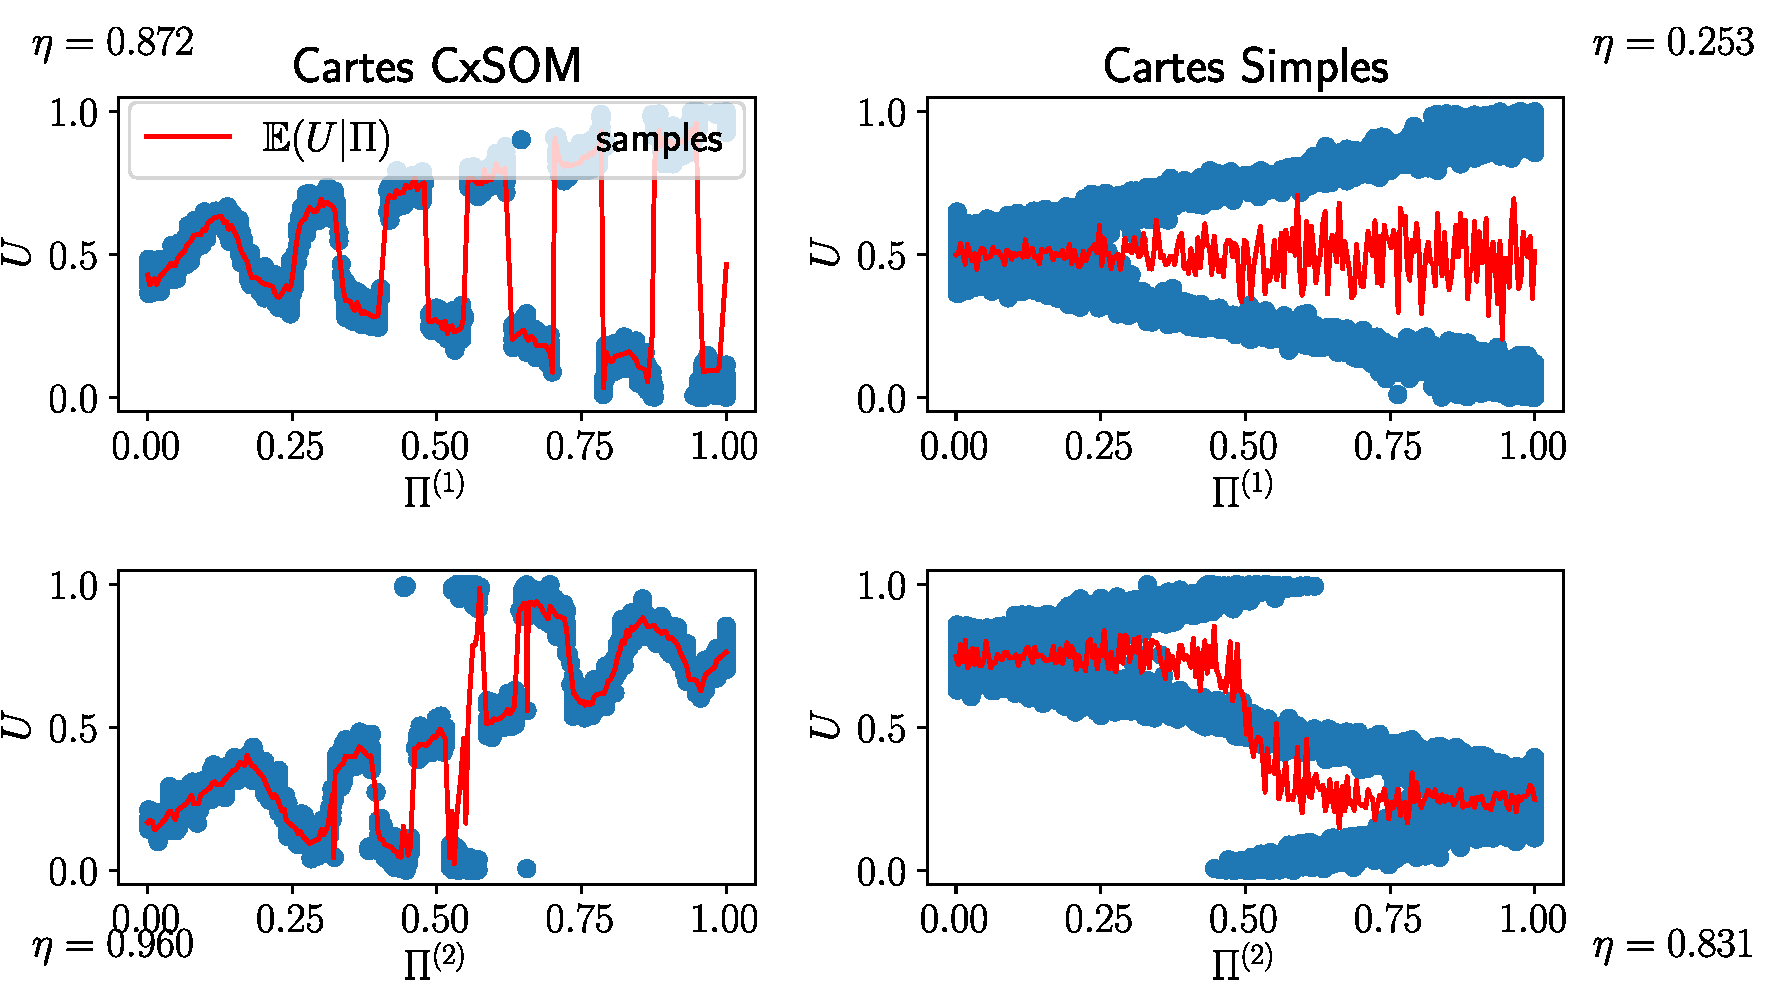
\includegraphics[width=\textwidth]{correlation_ratio_anneau_xp0.pdf}
    \caption{Tracé du ratio de corrélation sur cartes cxsom et cartes simples dans le cas ou les données sont bruitées.\label{fig:cr_bruit}}
\end{figure}

\begin{figure}
    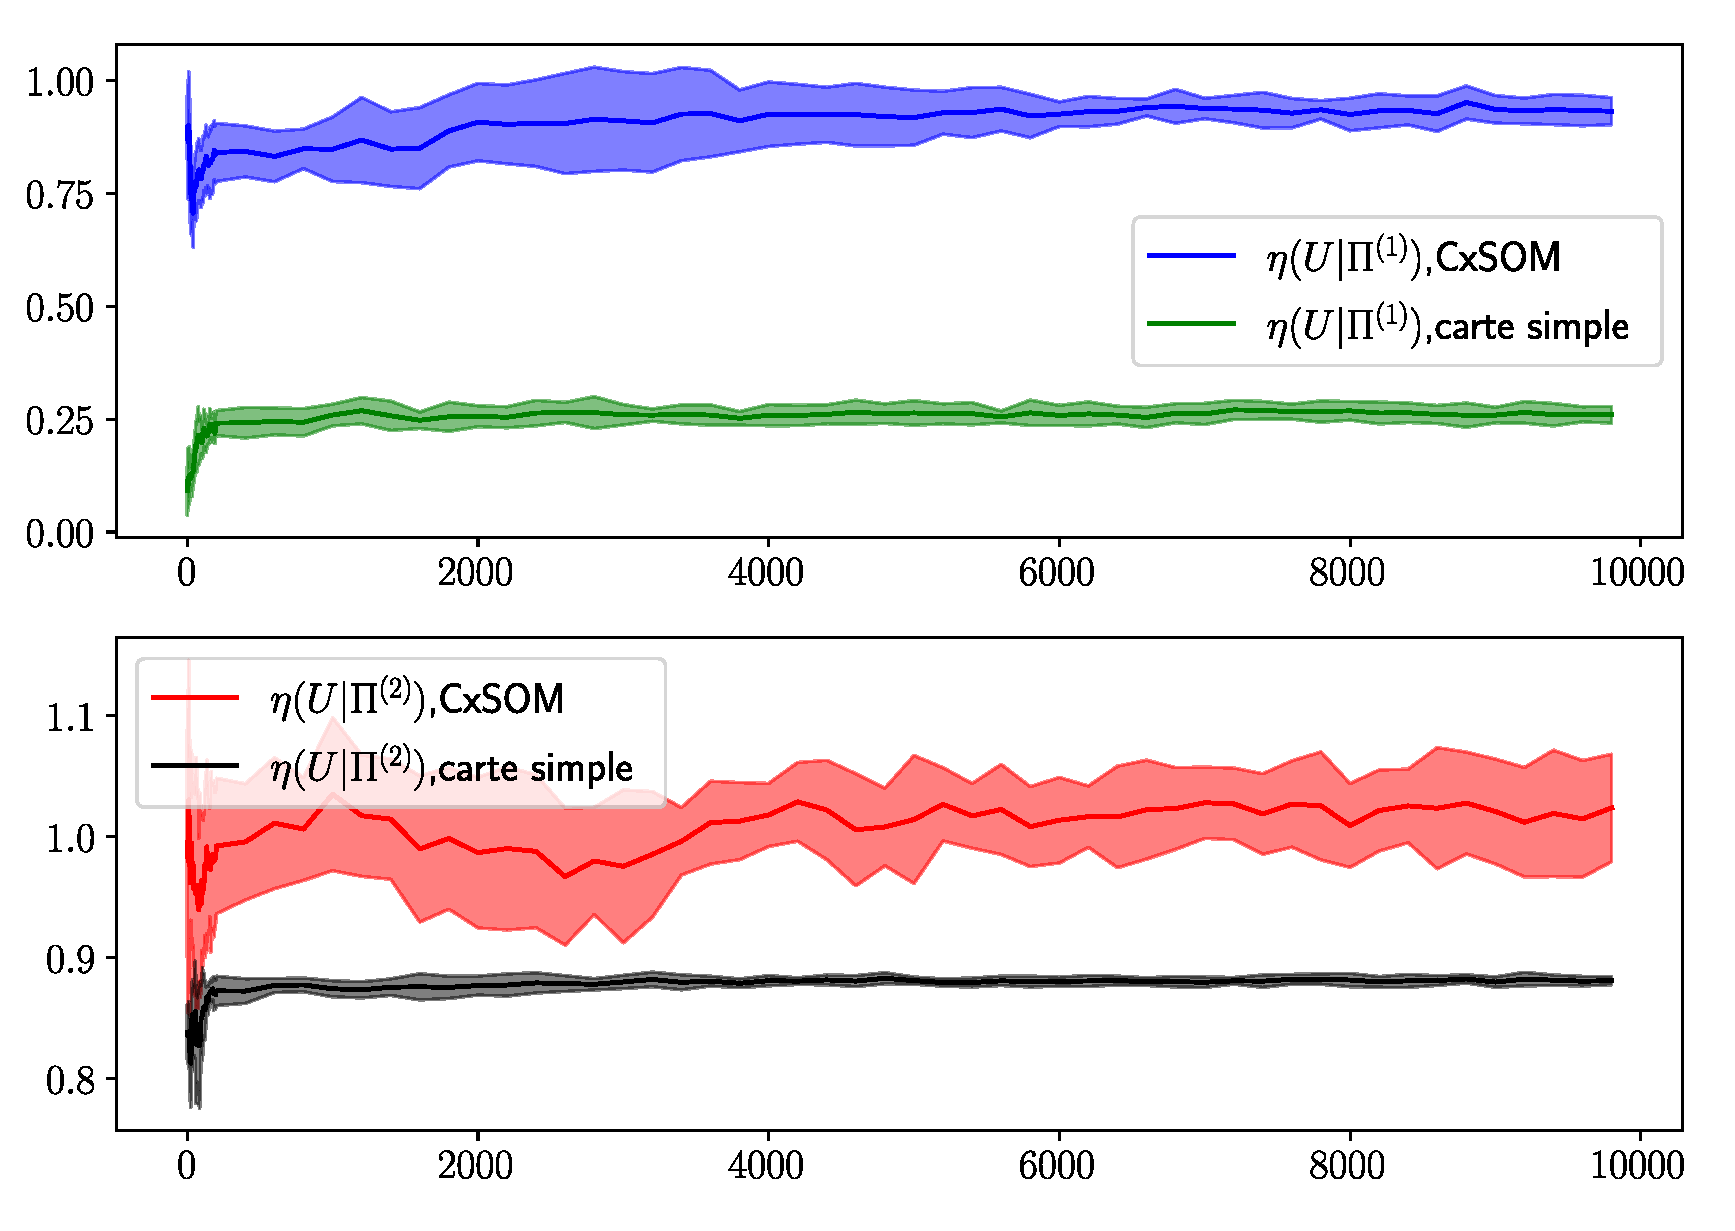
\includegraphics[width=\textwidth]{correlation_ratio_evolution_totale.pdf}
    \caption{Evolution du ratio de corrélation pendant l'apprentissage des cartes\label{fig:cr_evol}}
\end{figure}

\subsection{Discussion}
Bonne mesure de la relation existant entre $U$ et $\bmu$
Variable BMU discrète, variable U peut être continue
Très bien pour des dimensions plus grandes.

A mettre dans conclu générale: 
Néanmoins, il est montré (?) que  les variables restent sur des manifolds de dimension réduite - d'ou déjà l'intéret des cartes de kohonen et que ca marche. Donc les calculs de discretisation n'augmenteront pas de facon explosive au cours des dimensions ....


\section{Information mutuelle comme indicateur}

\subsection{Rappel des éléments de théorie de l'information}

Les notions d'\emph{entropie} et les valeurs associées, telle que l'\emph{information mutuelle} entre des distributions, sont des notions fondamentales de la théorie de l'information de Shannon. Ces quantités sont liées à la distribution d'une variable aléatoire.
L'entropie de Shannon d'une variable aléatoire $X$ à valeurs discrètes dans un ensemble $E_X$, de distribution $P_X$, est notée $H(X)$ et définie par la formule : 
\begin{equation}
H(X) = - \sum_{x \in E_X}{P_X(x)\textrm{log}(P_X(x))}
\end{equation}

Elle se mesure en $bit/symbole$ lorsque le logarithme est en base 2, ce qui est généralement utilisé. 
L'entropie est une mesure de la quantité d'incertitude, ou de surprise, sur la valeur de la variable aléatoire $X$. Si la la distribution de probabilité de $X$ est concentrée autour d'un point, l'entropie est faible : lors d'une réalisation de $X$, l'observateur est \emph{plutôt certain} du résultat. En revanche, l'entropie est maximale lorsque lorsque $X$ suit une distribution de probabilité uniforme.
L'entropie s'interpète également comme la quantité moyenne d'information à fournir, en bits, pour coder la valeur que prend la variable $X$.
De la même manière, on peut définir l'entropie conjointe de deux variables, qui est l'entropie de leur distribution jointe, et l'entropie conditionnelle, qui est l'entropie de leurs distributions conditionnelles.

Outre les entropies jointes et conditionnelles, l'existence d'une relation statistique entre deux variables aléatoires $X,Y$ à valeurs dans $E_X,E_Y$ se mesure par \emph{l'information mutuelle}. Elle se définit formellement par : 
\begin{equation}
 I(X,Y) = \sum_{x,y \in E_X,E_Y}{P_{XY}(x,y)\textrm{log}(\frac{P_{XY}(x,y)}{P_X(x)P_Y(y)})}
\end{equation}
Cette valeur mesure la quantité d'information moyenne partagée entre les distributions $X$ et $Y$: en moyenne, quelle information sur la valeur de $Y$ donne une valeur de $X$ et inversement, quelle information sur la valeur de $X$ donne une valeur de $Y$.

L'information mutuelle possède les propriétés suivantes:
\begin{enumerate}
\item $I(X,Y) = 0 \Leftrightarrow \textrm{X et Y sont indépendantes}$. L'information mutuelle peut être vue une mesure de la distance entre la distribution jointe de $(X,Y)$, $P(X,Y)$ et la distribution dans laquelle les deux variables sont indépendantes, $P(X)P(Y)$.
\item Elle s'exprime à partir de l'entropie : $I(X,Y) = H(X) + H(Y) - H(X,Y) = H(X) - H(X|Y) = H(Y) - H(Y|X)$
\item Elle est symétrique : $I(X,Y) = I(Y,X)$
\item Pour toute fonction $f$, $I(X,Y) \geq I(X,f(Y))$. L'égalité est atteinte si et seulement si $f$ est \emph{bijective}.
\end{enumerate}

Lors de l'analyse de CxSOM, on s'interroge sur l'information que portent les positions des BMUs $\bmu$ d'une carte sur le modèle d'entrée.
Les éléments de la carte ont été définis en termes statistiques~; on peut donc utiliser l'information mutuelle comme une représentation de l'information partagée entre la position du BMU d'une carte et la variable paramétrant le modèle d'entrée, $U$.

\subsection{Indicateur et estimation}

Nous avons présenté ci-dessus le ratio de corrélation, permettant d'évaluer le fait que $U$ est une fonction du BMU dans chacune des cartes. Cette propriété traduit le fait que le BMU d'une carte est sélectionné en fonction de tout le modèle et pas seulement de l'entrée externe.
Cet indicateur ne s'appuie cependant pas sur la distribution des positions $p$ dans la carte. Il traduit pas un apprentissage~: sa valeur reste en effet constante au cours de l'apprentissage.
Nous avons ainsi également exploré un indicateur basé sur l'information mutuelle pour l'évaluation de l'apprentissage~: le coefficient d'incertitude entre $U$ et $\bmu$.
Dans un premier temps, nous avons cherché à utiliser l'information mutuelle pour mesurer la même propriété que celle décrite par le ratio de corrélation, à savoir le fait que $U$ ets une fonction du BMU dans chaque carte. Nous avons publié le coefficient d'incertitude utilisé de cette façon en \cite{Gonnier2020ConsensusDS}.
Cet indicateur nous permet cependant d'évaluer d'autres propriétés de l'organisation des cartes. Nous détaillons ces deux aspects dans cette section.

\subsubsection{Définition de l'indicateur}

Nous cherchons à définir un indicateur de la relation fonctionnelle entre $U$ et $\bmu$. Cet indicateur prenne une valeur minimale lorsque $U$ n'a aucune relation avec $\bmu$, et augmente jusqu'à une valeur maximale lorsque $U$ est fonction de $\bmu$. Afin de pouvoir comparer les expériences entre elles, nous voulons définir un indicateur normalisé, dont la valeur est donc comprise entre $0$ et $1$.
Nous pouvons utiliser l'\emph{information mutuelle} $I(\bmu, U)$ pour évaluer l'information qu'une position du BMU d'une carte porte en moyenne sur la valeur de $U$, et $U$ sur le BMU. L'information mutuelle dépend de la quantité d'information portée par chaque distribution et se mesure en bit/symbole. 
Un indicateur normalisé nous permettra de comparer des expériences différentes. 
Nous choisissons de normaliser l'information mutuelle $I(\bmu,U)$  par la valeur maximale qu'elle peut prendre dans une expérience. Cette valeur maximale atteinte par $I(\bmu,U)$ est $H(U)$, atteinte lorsque $U$ est une fonction de $\bmu$.
En effet, par construction, $\bmu$ est une fonction de $U$ dans une carte de Kohonen~: l'algorithme est déterministe et une sortie est définie pour toute valeur de $U$. C'est à dire, $I(U,\bmu) = I (U, f(U))$.
Par propriété de l'information mutuelle, pour toute fonction $f$ et variables $X,Y$, $I(X,f(Y)) \leq I(X,Y) $. 
Donc, $I(U,\bmu) \leq I(U,U) = H(U)$
Cette valeur est atteinte si et seulement si $U$ et $\bmu$ sont en bijection, autrement dit, si et seulement si $U$ est aussi une fonction de $\bmu$.

Nous définissons donc un indicateur de la relation fonctionnelle existant entre $U$ et $\bmu$ comme:
\begin{equation}
I_x(U|\bmu) = \frac{I(\bmu,U)}{H(U)}
\end{equation}
Ce coefficient n'est pas symétrique et mesure l'information portée par le second terme sur le premier, relativement à la valeur maximale qu'il peut porter ($H(U)$). On a $I_x(U|\bmu) \in [0,1]$. Cette valeur est une variante normalisée de l'information mutuelle appelée le \emph{coefficient d'incertitude} entre $U$ et $\Pi$ et introduite par Theil en~\cite{Theil1961EconomicFA}.
Il vaut 1 lorsque $U$ est une fonction de $\bmu$ dans la carte considérée, et $0$ lorsque les deux distributions sont indépendantes. Cette relation fonctionnelle entre $U$ et $\bmu$ est bien la propriété qu'on souhaite mesurer.

%TODO : développer ce point : information portée par plus de variables !
%TODO : calculer et comparer les valeurs pour le cas du cercle.

% Ce coefficient peut être élargi à plus de variables: on peut calculer $I_x(U | (\bmu\m{1},\bmu\m{2},\bmu\m{3}))$ pour 3 cartes, en considérant la variable jointe $(\bmu\m{1},\bmu\m{2},\bmu\m{3})$.
% Plus largement, pour prouver que l'archictecture a appris un modèle, on souhaite que $I_x(U|\bmu\m{1},\cdots,\bmu\m{k})$ soit le plus proche possible de 1.
% Cet indicateur permet de comparer des expériences par des valeurs numériques, sans passer par des tracés.
\subsubsection{Estimation de l'indicateur}

L'information mutuelle et l'entropie sont des grandeurs définies à partir de la distribution des variables aléatoires. Ces distributions, dans notre cas, ne sont pas connues, nous devons donc estimer ces quantités à partir des échantillons de données.
La méthode classique d'estimation de l'information mutuelle et de l'entropie est la méthode dite des \emph{histogrammes}.
Cette méthode s'appuie sur une estimation de la distribution des variables $U$,$\bmu$ et la distribution de la variable jointe $(U,\bmu)$ en discrétisant chacune des variables.
Cette méthode est représentée en figure~\ref{fig:binning}. Les variables $U$ et $\bmu$ sont discrétisées en \emph{boîtes} de centres $x_k$ et $y_k$ choisis.
Une distribution est alors estimée par: 
$$P(U = x_i) = \frac{n_{xi}}{N} $$ où $n_{xi}$ est le nombre d'échantillons de $U$ tombant dans la boîte de centre $x_i$ et $N$ le nombre de points. Le même procédé est réalisé pour $\bmu$ et $(U,\bmu)$. La précision de l'estimation peut être améliorée en choisissant des tailles de boîtes variables; nous utilisons ici la méthode simple avec des boites de taille fixe.
Pour des variables à valeur dans $[0,1]$, les centres sont définis par $x_k = \frac{k}{M}+\frac{1}{2M}$, avec $M$ le nombre de boîtes.
Cette discrétisation permet d'estimer les trois termes d'entropie $\hat{H}(\bmu,U)$, $\hat{H}(U)$ et $\hat{H}(\bmu)$ et d'en tirer l'information mutuelle normalisée:
\begin{equation}
    \hat{I_x}(U,\bmu) = \frac{\hat{H}(U) + \hat{H}(\bmu) - \hat{H}(U,\bmu)}{\hat{H}(U)}
   \end{equation}

La valeur de cet indicateur dépend de la résolution choisie pour l'histogramme. L'estimateur  par histogramme converge vers la valeur théorique de l'information mutuelle continue lorsque la taille des boites tend vers 0, sous réserve que les densités de probabilité existent pour chaque variable. Plus la taille des boîtes est petite, plus le nombre de points disponible pour l'estimation doit augmenter.
Notons que la méthode par histogrammes est limitée quand la dimension des entrées augmente.
Le nombre d'échantillons disponibles pour l'estimation doit augmenter exponentiellement avec la dimension des variables pour éviter le phénomène de "boîtes vides": à cause de la dispersion des données, de nombreuses boîte $(x_j,y_i)$ ne contiendront pas de points alors qu'elles auraient dû en contenir selon leur distribution; l'estimation de la distribution en ce point sera alors nulle, et l'estimation de l'indicateur faussée.

Une deuxième méthode généralement utilisée pour l'estimation de l'information mutuelle est l'estimateur par KNN (K-nearest neighbors) de Kraskov \cite{2004kraskov}. 
Cet estimateur ne passe pas par l'estimation de la densité de probabilité, contrairement aux histogrammes, mais estime directement les entropies et l'information mutuelle.
Le découpage de l'espace se fait en recherchant, pour un couple $(X,Y)$ les k plus proches voisins. Une information mutuelle locale est calculée dans cette zone de l'espace, suivant une formule permettant d'approximer les différences de logarithme par la fonction digamma $\psi$ : 
$$i_j(X,Y) = \psi(k) - \psi(n_{x_j} + 1) - \psi(n_{y_j} +1) + \psi(N)$$
Cette information mutuelle locale est ensuite moyennée sur l'ensemble des points: 
$$\hat{I}(X,Y) = \psi(k) - \langle\psi(n_{x_j} + 1) + \psi(n_{y_j} +1)\rangle + \psi(N)$$
Pour estimer $I_x(X|Y)$, on estimera $I(X,Y)$ et $H(Y)$, en notant que $H(Y) = I(Y,Y)$.
L'estimateur de Kraskov est plus précis que l'estimateur par histogrammes et est moins sensible aux paramètres choisis pour son estimation, en l'occurrence le nombre de voisins considérés. Il est notamment plus performant que l'approche par histogrammes en grande dimension.

En considérant ces deux méthodes d'estimation, on pourrait conclure qu'utiliser un estimateur peu biaisé tel que celui de Kraskov est plus pertinent car il permet une estimation précise de la quantité théorique qu'est le coefficient d'incertitude.
Cependant, nous ne nous intéressons pas réellement à la valeur théorique de cet indicateur. Une dispersion locale est observée sur les valeurs de $U$: un BMU encode non pas une valeur précise de $U$ mais une petite zone de valeurs. Cela nous amènera à privilégier la méthode par histogrammes, ce que nous détaillons au paragraphe suivant.

\begin{figure}
    \begin{minipage}{0.4\textwidth}
    \centering
    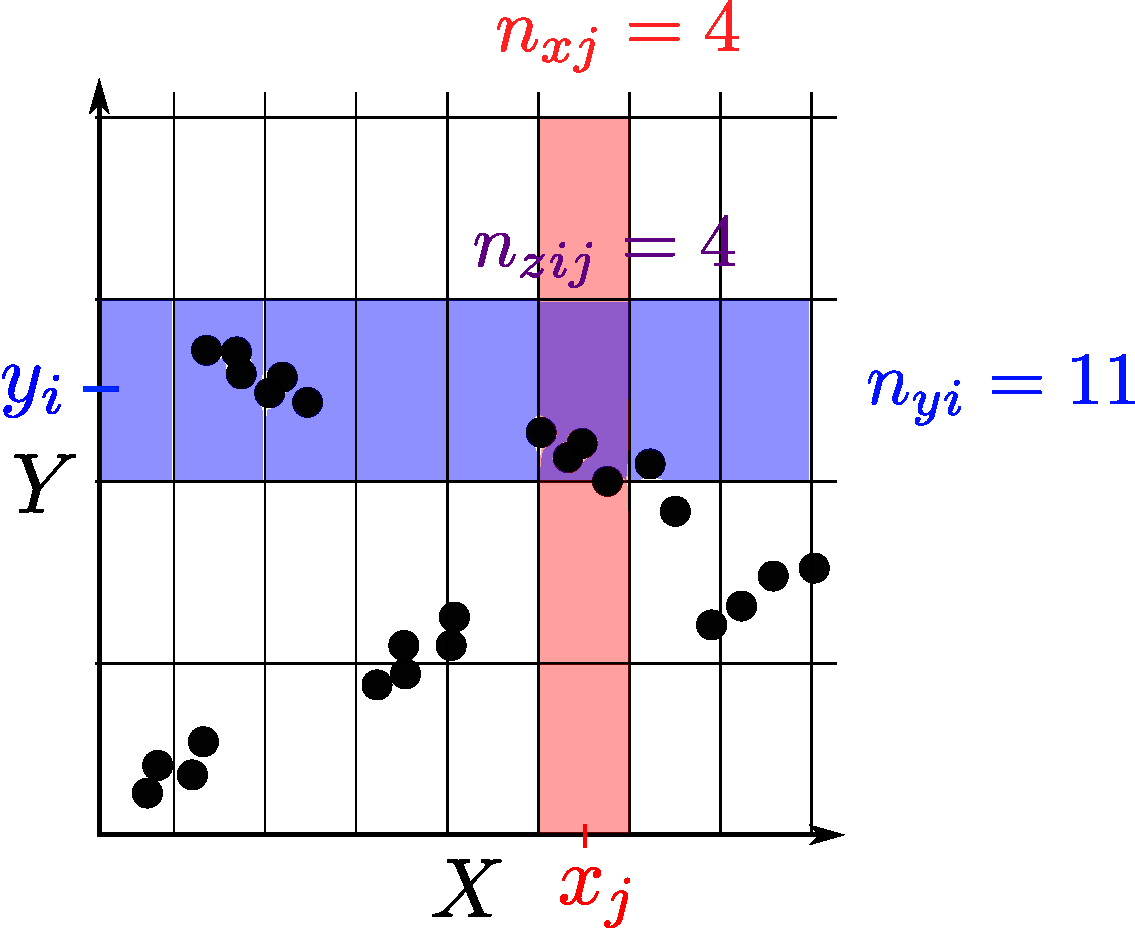
\includegraphics[width=\textwidth]{boxes}
    \caption{Méthode par histogrammes pour estimer les distributions des variables $U$ et $\bmu$. Les distributions sont estimées à partir de $n_{xj}$, $n_{yi}$ et $n_{zij}$, puis les valeurs de l'entropie $H$ et l'information mutuelle $I$ calculées.}
    \label{fig:binning}  
    \end{minipage}
    \hfill
    \begin{minipage}{0.4\textwidth}    
            \centering
            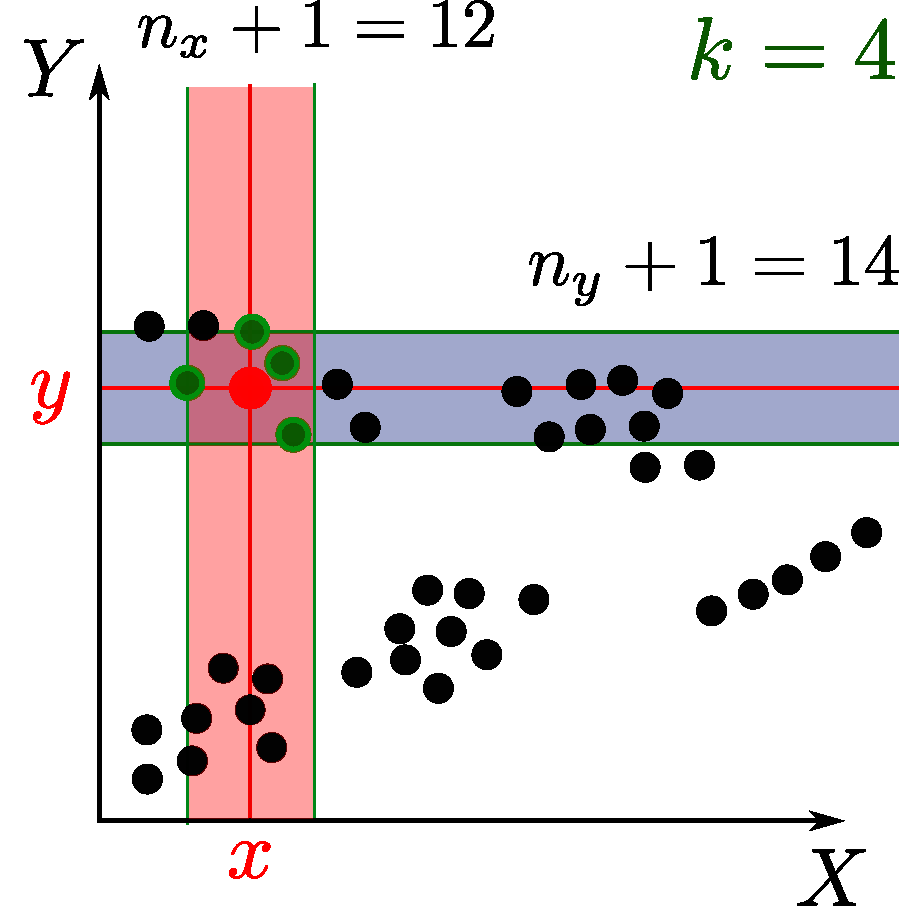
\includegraphics[width=0.8\textwidth]{kraskov.pdf}
            \caption{Découpage en KNN de Kraskov pour estimer l'entropie et l'information mutuelle des variables $X$ et $Y$. Les plus proches voisins du point rouge sont trouvés, en vert, et le processus est répété sur tous les points. Les valeurs de $n_x$ et $n_y$ permettent d'estimer directement l'entropie.\label{fig:kraskov}}
            
    \end{minipage}
    \end{figure}


L'information mutuelle mesure l'existence d'une relation statistique, linéaire ou non linéaire, entre les deux distributions. La figure~\ref{fig:exemple-limite} présente deux exemples de relations entre les variables $U$ et $\bmu$.
Dans le cas de gauche, la relation se rapproche d'une relation fonctionnelle, qu'on souhaite dans le cas de CxSOM, mais cette relation est bruitée. Dans le cas de droite, la relation n'est pas une fonction, mais elle est "précise": une valeur de $\bmu$ correspond à deux valeurs de $U$ et pas plus.
Nous avons calculé l'indicateur $I_x$ sur les deux distributions, estimé avec la méthode des histogrammes de Kraskov. La méthode de Kraskov est considérée comme donnant une valeur plus proche de la valeur théorique de l'information mutuelle que la méthode par histogrammes. 

Dans le cas de gauche, la méthode de Kraskov donne un coefficient d'incertitude assez faible. En effet, une valeur de $\bmu$ correspond à tout un intervalle de valeurs pour $U$. Sur le cas de droite, sa valeur est plus haute. En effet, une valeur de $\bmu$ correspond à deux valeurs de $U$, ce qui donne plus d'information que dans le premier cas de figure. Ce n'est pas ce qu'on veut mesurer dans CxSOM: le bruit est accepté, tant que la relation se rapproche d'une fonction.
La méthode des histogrammes permet d'ignorer ce bruit en prenant une taille de découpe plus grande pour $U$. Grâce à la méthode par histogrammes, l'indicateur normalisé possède une valeur forte, proche de 1 dans le cas de la droite, et plus faible dans le cas du cercle.

Dans le cas de CxSOM nous ne souhaitons ainsi pas une estimation précise de l'information mutuelle.
Le but de l'indicateur est de mesurer une relation de type fonction entre $U$ et $\bmu$.
Cette relation peut être bruitée et imprécise localement: on cherche à mesurer si une valeur de $\bmu$ correspond à \emph{un unique} intervalle de $U$, et non plusieurs comme dans le cas d'une carte simple, dans laquelle deux valeurs de $U$ sont codée par une position de BMU, voir figure~\ref{fig:upi_chap4}.
Nous utiliserons donc l'indicateur $I_x$ pour CxSOM en l'estimant par la méthode des histogrammes, avec un découpage large pour $U$. Cette façon d'estimer permettra de gommer la dispersion locale sur la valeur de $U$ pour mesurer uniquement la relation fonctionnelle existant entre $U$ et $\bmu$.

L'indicateur $I_x$ doit ainsi être considéré plutôt comme un indicateur s'inspirant du coefficient d'incertitude que comme une estimation précise de cette valeur. 
C'est cette estimation large qui nous permettra d'évaluer qu'une carte a dissocié les positions de ses BMUs en fonction de $U$ et non seulement de son entrée externe.
L'estimation du coefficient par la méthode de Kraskov donne quant à elle une valeur précise de la quantité statistique qu'est le coefficient d'incertitude entre $U$ et $\bmu$.
Nous pouvons considérer cette quantité comme un deuxième indicateur différent de $I_x$, que nous noterons $UC$, étant donné qu'il s'agit d'une valeur précise du coefficient d'incertitude. 

\begin{figure}
    \centering
    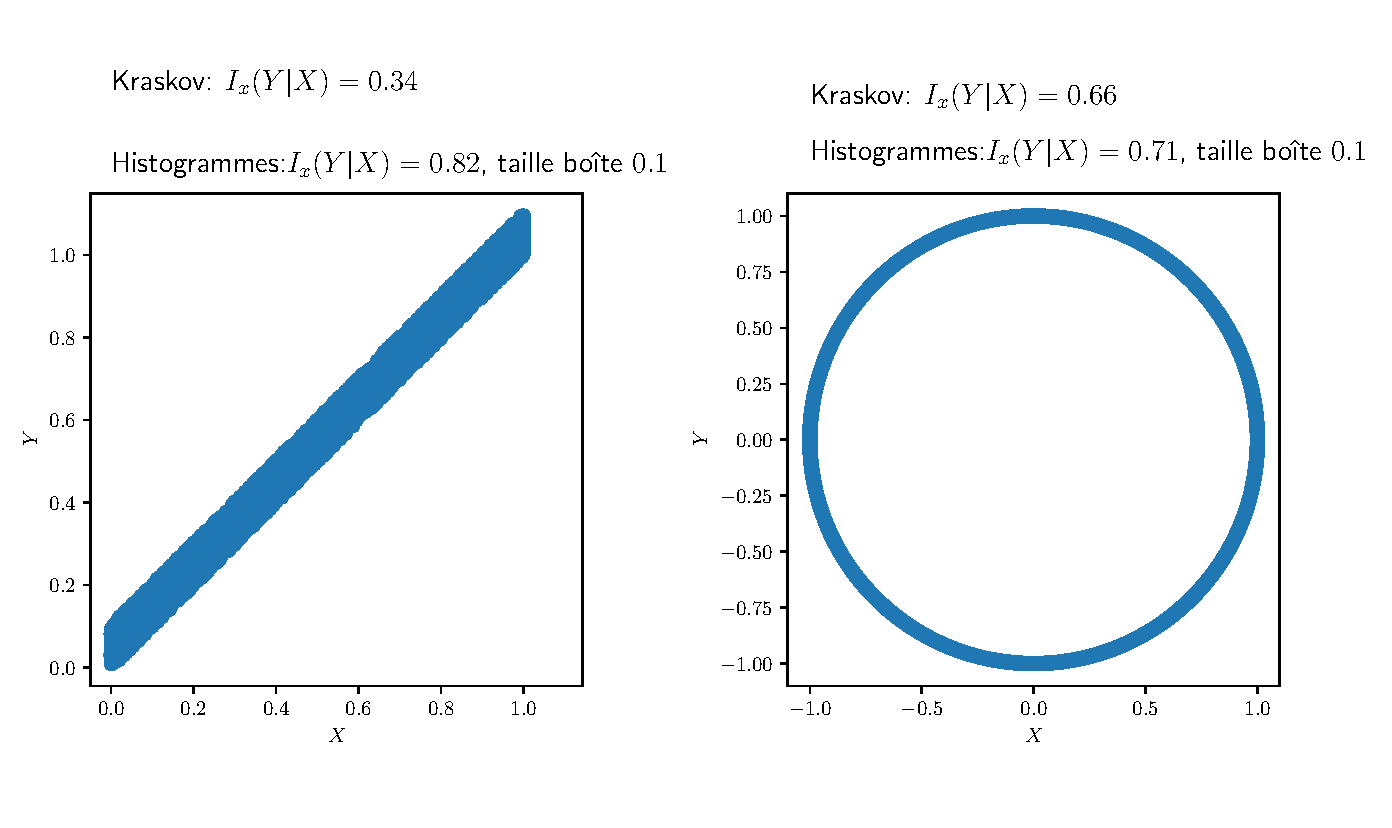
\includegraphics[width=0.75\textwidth]{comparaison_binning_kraskov.pdf}
    \caption{Comparaison du calcul de l'indicateur $I_x$ sur deux distributions. A gauche, la relation entre $Y$ et $X$ se rapproche d'une fonction, mais bruitée. A droite, la relation n'est pas fonctionnelle, mais de telle sorte qu'une valeur de $X$ correspond au maximum à deux valeurs de $Y$. Lorsqu'on calcule l'indicateur avec la méthode très granulaire de Kraskov, cet indicateur est plus élevé dans le cas de droite que de gauche: en effet, le calcul ne prend pas en compte si les points sont condensés ou éloignés. Pour que l'indicateur nous informe correctement sur l'aspect fonctionnel de la relation entre $X$ et $Y$, il faut enlever manuellement le bruit. Avec la méthode par histogrammes, on prend une taille de boîte de $0.1$ selon $Y$. Dans ce cas, l'indicateur est bien plus élevé à gauche, ou $Y$ se rapproche d'une fonction de $X$, que à droite. \label{fig:exemple-limite}}
   
    \end{figure}


\subsubsection{Application de l'indicateur $I_x$ au cas d'exemple multimodal simple}

Nous avons défini deux indicateurs à partir du coefficient d'incertitude. Premièrement, $I_x$, coefficient estimé par histogrammes avec de larges intervalles dans le découpage de $U$, permettant d'évaluer si $U$ est une fonction de $\bmu$, et autorisant une variation locale de $U$ pour une position de BMU.
En second lieu, $UC$, le coefficient d'incertitude estimée de façon précise avec une méthode d'estimation telle que les KNN de Kraskov.
Dans les deux cas, les indicateurs $I_x(U|\bmu)$ et $UC(U|\bmu)$ valent 1 lorsque $U$ est une fonction parfaite de $\bmu$. Cependant, $I_x$ nous permet de ne pas prendre en compte la dispersion des données au niveau d'une valeur de $U$ et permet d'évaluer si les BMUs sont différenciés selon $U$ dans une carte. 
$UC$ nous renseigne sur la valeur théorique du coefficient d'incertitude.

Le fait d'utiliser un indicateur numérique permet de tracer l'évolution de cet indicateur au cours de l'apprentissage des cartes.
Nous traçons cette évolution au cours de l'apprentissage dans un système de deux cartes apprenant sur le cercle en deux dimensions, l'exemple présenté au chapitre précédent.
Nous chercherons à vérifier que $I_x$ reflète bien la qualité de l'apprentissage dans une carte, puis nous utiliserons $UC$ pour évaluer l'information réellement portée par les cartes.

Pour cette expérience, une phase de test sur 5000 entrées est réalisée à intervalles réguliers lors de l'apprentissage, en utilisant le même jeu d'entrées pour chaque test. Chaque phase de test donne alors un ensemble d'entrées $\inpx\m{1}, \inpx\m{2}, U$ et un ensemble de réponses des cartes $\bmu\m{1}, \bmu\m{2}$. On peut alors estimer $I_x(U|\bmu\m{1})$ et $I_x(U|\bmu\m{2})$ sur chaque itération considérée et tracer la courbe de l'évolution de l'indicateur au long de l'apprentissage. 
Ces calculs sont réalisés sur 100 apprentissages séparé, prenant des entrées d'apprentissage aléatoires sur le même cercle. Les cartes sont initialisées à des poids aléatoires différents au début de chaque apprentissage. 
Les tracés représentent la moyenne, à chaque pas de temps, des indicateurs considérés au pas de temps $t$.

Nous étudions d'abord l'évolution de $I_x$, calculé en discrétisant l'espace par la méthode des histogrammes.
On choisit de découper les valeurs de $U$ en 50 boîtes, et en 500 pour $\bmu\m{i}$: comme soulevé en section précédente, il est nécessaire d'utiliser un intervalle plus large pour les valeurs de $U$, afin de ne pas prendre en compte la dispersion des points au niveau local. Le tracé obtenu est tracé en figure~\ref{fig:MI_evol}.

Nous comparons les valeurs obtenues pour une carte de CxSOM à celles d'une carte simple apprenant sur les mêmes entrées $\inpx\m{1}$ ou $\inpx\m{2}$.
On s'attend à ce que l'information soit plus élevée pour la carte au sein de CxSOM que la carte seule. Cela montrera qu'une carte porte de l'information sur son entrée externe mais également sur le modèle global $U$, donc sur l'autre entrée.
On s'attend également à ce que cette valeur atteigne 1, ce qui montrerait qu'une seule carte porte de l'information sur tout le modèle~: $U$ est une fonction de $\bmu$ dans chaque carte.

L'observation du tracé montre que les quantités $I_x(U|\bmu\m{1})$ et $I_x(U|\bmu\m{2})$ sont bien toutes deux plus élevées à chaque moment de l'apprentissage que dans le cas ou les cartes sont séparées; la valeur s'approche de 1 dans le cas de CxSOM.
Ces quantités augmentent au cours de l'apprentissage, traduisant bien un gain d'information des cartes sur le modèle au cours de l'apprentissage.

Nous pourrons donc utiliser $I_x$ comme indicateur d'une relation fonctionnelle entre $U$ et $\bmu$ dans chaque carte, en choisissant bien la taille de discrétisation pour $U$ lors de l'estimation. La taille de l'intervalle doit être assez élevée pour englober le bruit local des données, mais suffisamment faible pour détecter une séparation entre deux intervalles de $U$ codé par une même position de BMU.

\begin{figure}
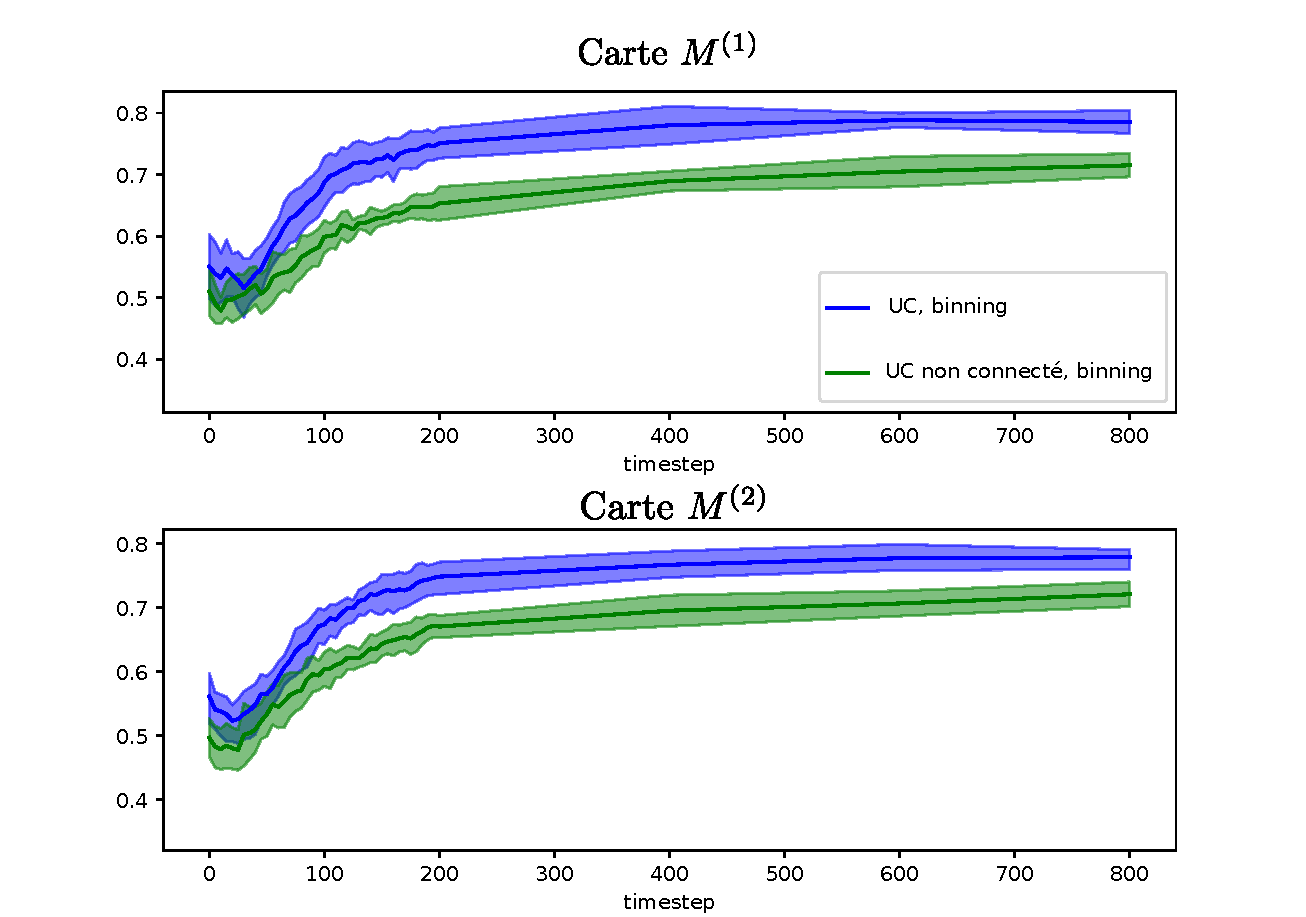
\includegraphics[width=\textwidth]{evolution_MI_binning}
\caption{Evolution de l'information mutuelle normalisée $I_x(U|\bmu)$ dans chaque carte au long de l'apprentissage. La courbe bleue correspond à $I_x(U|\bmu)$ dans l'architecture de cartes $M\m{1}$ et $M\m{2}$. On compare cette évolution à l'évolution de l'information d'une seule carte apprenant sur les mêmes entrées $X$ ou $Y$, sans être connectée.}
    \label{fig:MI_evol}
\end{figure}

\subsection{Discussion}

Dans ce cas d'application, le coefficient d'incertitude mesure bien l'information portée par $\bmu$ sur la variable $U$. Cependant, il ne permet pas de mesurer correctement l'aspect fonctionnel de la relation. Nous privilégierons donc le ratio de corrélation pour mesurer si les BMUs sont bien séparés en fonction de la variable multimodale $U$ dans chaque carte.

Cependant, cet indicateur permet de mesurer quelle information la distribution des BMUs porte sur la distribution de U. 

\subsection{Utilisation du coefficient d'incertitude comme mesure de l'information apprise par le modèle}

Nous sortons de l'étape de validation de l'indicateur $I_x$ cherchant à évaluer une relation fonctionnelle autorisant le bruit local, pour étudier l'évolution du coefficient d'incertitude $UC$ entre les distributions de $U$ et de $\bmu$, estimée cette fois de façon précise, avec la méthode de Kraskov.
Le but est de comparer l'évolution du coefficient d'incertitude dans une carte CxSOM avec l'évolution dans une carte simple. Cet indicateur représente maintenant vraiment le taux l'information portée par une valeur $\bmu$ sur une valeur de $U$.

En figure~\ref{fig:MI_evol_total}, nous tracons l'évolution de $UC$.
Sur les tracés, il converge vers une valeur similaire à la fin de l'apprentissage pour la carte simple que pour la carte au sein d'une architecture CxSOM (tracés rouges et noirs). La valeur de $UC$ pour une carte dans CxSOM est même plutot inférieure à la valeur prise dans une carte simple.
Ce résultat est étonnant: cela signifie donc que la carte au sein de CxSOM n'a pas plus d'information sur le modèle qu'une carte isolée. Ce résultat va également à l'encontre de ce qu'on observe sur l'évolution de l'information mutuelle calculée par les histogrammes, dans laquelle une différence franche est observée entre la carte isolée et la carte au sein de l'architecture.

Proposons une explication.
On observe que l'information $UC(U|\bmu)$ tend vers une même valeur dans CxSOM et dans une carte isolée quand on la calcule avec l'estimateur de Kraskov, qui est proche de la valeur théorique de l'indicateur. Cela signifie qu'on a effectivement la même quantité d'information sur $U$ avec le BMU dans la carte isolée que dans CxSOM. Simplement, cette information n'est pas répartie de la même façon dans les deux expériences.
Dans une carte isolée, le niveau de quantification vectorielle qu'on effectue sur $\inpx$ est très précis: lorsqu'on présente une entrée $\inpx$ à la carte, le poids du BMU sera très proche de cette valeur $\inpx$. Or, la connaissance de $\inpx$ donne déjà beaucoup d'information sur le modèle $U$.
Dans CxSOM, on perd ce niveau de quantification sur $\inpx$, ce qu'on a observé en figure~\ref{fig:erreur}. On perd donc de l'information sur $\inpx$. 
Le fait que l'information mutuelle normalisée prenne la même valeur dans les deux expériences traduit alors qu'on a perdu de l'information sur l'entrée $\inpx$ par rapport à la carte isolée, avec la perte de précision, mais qu'on a en même temps gagné de l'information sur le modèle d'entrée, par la séparation selon $U$. Le fait que les deux évolutions de $I_x$, pour chaque expérience, convergent vers la même valeur montre qu'on est dans une situation de compromis: on gagne de l'information sur le modèle $U$, au détriment de l'information apprise sur l'entrée externe.
Ce comportement sera à valider sur d'autres modèles d'entrées.

C'est donc le fait de discrétiser grossièrement la distribution de $U$ qui permet de mesurer le gain d'information sur le modèle complet, sans prendre en compte le fait que la précision sur l'entrée externe est affaiblie. 
La comparaison de la valeur précise du coefficient d'intertitude, estimé par Kraskov, entre la carte simple et la carte dans CxSOM nous indique que la quantité d'information totale gagnée par une carte reste similaire dans le cas d'une carte simple qu'une carte dans CxSOM; elle est simplement répartie différemment entre les deux expériences.

\begin{figure}
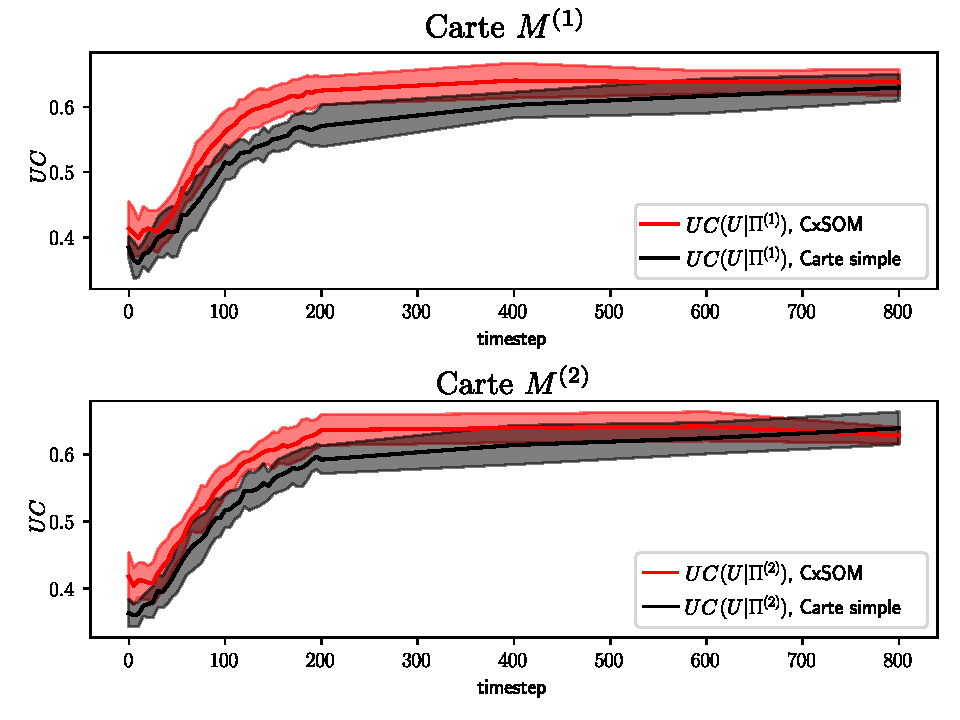
\includegraphics[width=\textwidth]{evolution_MI_K}
\caption{Evolution de $UC(U|\bmu)$ dans chaque carte au long de l'apprentissage, estimé par la méthode de Kraskov.\label{fig:MI_evol_total}}
\end{figure}
\section{Conclusion}

Afin d'extraire des comportements d'une architecture de cartes, nous modélisons les éléments des cartes comme des variables aléatoires et l'étape de test comme l'échantillonnage d'une variable jointe. Nous introduisons notamment, dans le cas des exemples artificiels, une variable cachée $U$ non présentée comme entrée à la carte, portant toute l'information sur le modèle d'entrées.
La représentation par échantillonnage et variable aléatoire permet de mieux comprendre les mécanismes des cartes, ceux ci ne reposant plus directement sur les courbes de poids.

Nous utiliserons donc quatre représentations des cartes dans la suite de cette thèse, toutes définies à partir d'un échantillon de test.
Le tracé du poids du BMU en fonction de l'entrée externe permet d'évaluer comment chaque carte extrait une représentation de son espace d'entrée.
La représentation cartographique des entrées selon le BMU de chaque carte fait apparaître des zones mortes dans les cartes CxSOM et affiche les valeurs préférentielles d'entrées selon leur BMU. Cette représentation met en lumière un comportement émergeant de l'exemple à deux cartes: de façon auto-organisée, chaque carte définit des zones de BMUs correspondant à intervalle de valeurs $(\inpx\m{1},\inpx\m{2})$, et non seulement $\inpx\m{1}$. Cette représentation fait également apparaître une notion d'organisation selon un indice primaire sur les poids externes, et secondaire grâce aux poids contextuels. Nous étudierons plus extensivement ce comportement dans la partie suivante grâce à cette représentations.
Afin d'évaluer la façon dont un BMU traduit le modèle d'entrée, nous traçons la variable cachée $U$ en fonction du BMU d'une carte $\bmu\m{i}$.
L'apprentissage du modèle d'entrée se traduit alors par l'observation d'une \emph{relation fonctionnelle} entre $U$ et $\bmu$ dans chaque carte.
Enfin, nous proposons une représentation du dépliement de chaque carte dans l'espace de toutes les entrées en traçant les poids des BMUs de chaque carte, ordonnés selon les BMUs d'une des cartes. Cette représentation apporte une vision globale de la façon dont une carte encode le modèle d'entrées.
Ces représentations permettront d'étudier plus en détail les comportements observés dans l'exemple illustratif. Cette étude sera traitée au chapitre~\ref{chap:analyse}.

Même avec des représentations adaptées, l'analyse d'architectures comportant de nombreuses cartes ne peut pas simplement s'effectuer à l'aide de graphiques, qui deviendraient trop complexes. La comparaison d'un grand nombre d'expériences est aussi difficilement réalisable graphiquement.
Cette difficulté de représentation et le besoin de comparer des expériences soulève la nécessité de définir une valeurs indicatrice du fonctionnement de la carte, que nous proposerons dans le chapitre suivant.


% \comment{Correlation ration : mesure de dépendance fonctionnelle
% Débruitage de l'IM : répétition de l'expérience et moyenne ?}
% \draft{Le ration de corrélation traduit mieux que le coefficient d'incertitude la dépendance fonctionnelle entre le modèle et le BMU. Cependant, à l'inverse de l'information mutuelle, une relation non fonctionnelle mais précise (telle que l'exemple du cercle de la figure~\ref{fig:exemple-limite}) entre les variables aura un score très faible. Ce n'est pas non plus voulu. 

% Il semble que l'information mutuelle reste le moyen le plus prometteur et le plus général de mesurer la relation entre les éléments des cartes. Dans le cas une dimension, on observe qu'on veut tendre vers U fonction du BMU; on connait mal le comportement recherché en dimension plus grande (cartes 2D, entrées de grande dimension). L'information mutuelle laisse donc l'opportunité à plus d'états d'organisation des cartes de l'architecture d'avoir un bon score. La meilleure perspective serait donc de pouvoir calculer le coefficient d'incertitude sur des échantillons provenant de données non bruitées, ou de pouvoir séparer le bruit des données lors du calcul du coefficient.
% Dans cette optique, l'estimateur par histogrammes permet de réduire l'effet du bruit, en choisissant correctement les tailles de boîtes. L'utilisation histo versus Kraskov reste donc à discuter.
% Dans le cas ou le modèle d'entrée est connu, calculer les réponses des cartes sur des jeux de données non bruitées générées artificiellement, après apprentissage sur un jeu de données réelles et bruitée, est une solution. Si le modèle n'est pas connu, des méthodes statistique de réduction de bruit peuvent être imaginées.} 

% \draft{
% \section{Prédiction d'entrée}

% Au sein d'une architecture de cartes, il est possible de ne pas présenter à une ou plusieurs cartes de l'architecture leur entrée externe $\inpx\m{i}$. Dans ce cas, une best matching unit peut quand même être calculée par leurs entrées contextuelles. Le poids de cette best matching unit peut alors être vu comme une prédiction de l'entrée manquante. Cette capacité de prédiction peut être à la fois vue comme une application possible de l'architecture, mais aussi comme une façon de représenter \emph{ce que les autre cartes connaissent d'une autre}. Tracer les prédictions d'une carte est donc un indicateur de la façon dont une architecture a appris des relations. 


% \comment{
% 2 parties dans estimation/perspectives : 
% d'une part, questionnement sur l'estimation des données bruitées par exemple - pas besoin de proposer des solutions si elles ne sont pas testées ? 
% Et parler de l'estimation en grande dimension : ce n'est pas forcément le pb ici. Donc pas la peine...
% }
% }

\ifSubfilesClassLoaded{
    \printbibliography
    %\externaldocument{../main.tex}   
}{}
\end{document}